\section{楽器を持って音を出そう}
\begin{center}
\begin{tabular}{|lcl|}
\hline
この章の修了課題 & : & 1. 正しく楽器・弓を持てる\\
                 &   & 2. 開放弦の練習(\ref{open2})を暗譜で弾ける\\
\hline
\end{tabular}
\end{center}

\subsection{楽器の運び方}



\subsection{楽器の置き方}
楽器を置くときは左側を下にして、なるべく椅子などに立てかけるようにしましょう\addtocounter{figure}{1} (図\thefigure、図\addtocounter{figure}{1}\thefigure)。右側を下にするのは\ruby{魂}{こん}\ruby{柱}{ちゅう}\footnote{楽器内部で表板と裏板に挟まれている棒状の部品。{\it f}字孔から楽器内部を覗くと確認できる。}の安定に良くありません。

\begin{minipage}{200pt}
\addtocounter{figure}{-1}
\begin{center}
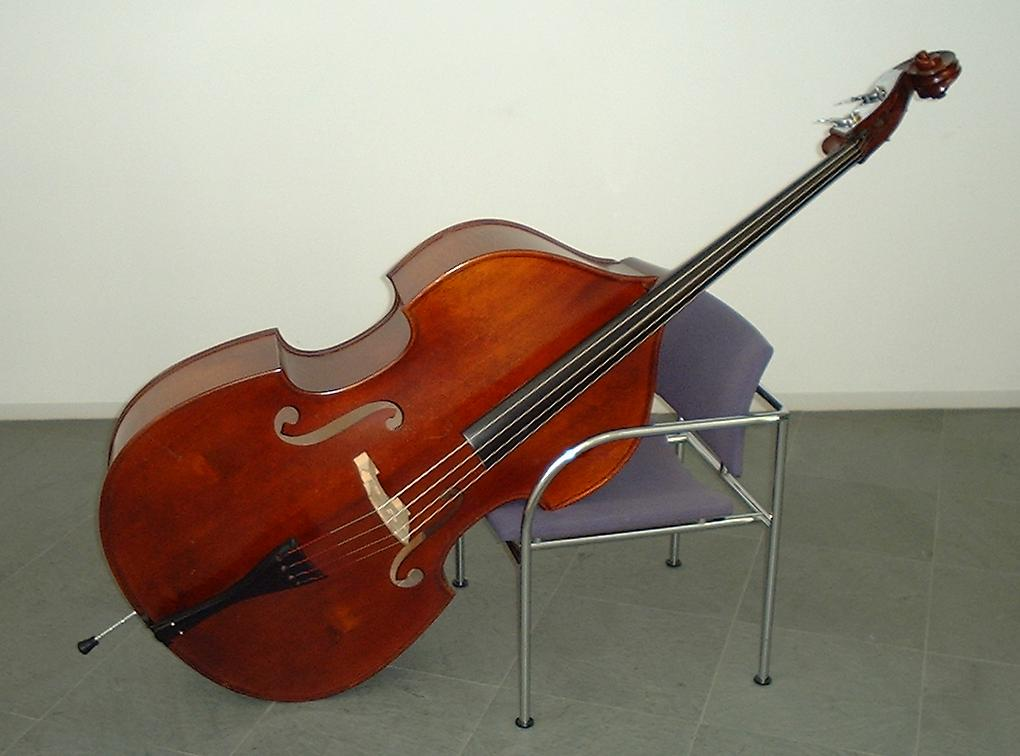
\includegraphics[height=2.7cm]{Pics/Instrument/on_chair.epsi}\\
{\small 図\thefigure : 椅子に立てかける場合\\}
\end{center}
\end{minipage}
\hfill
\begin{minipage}{200pt}
\addtocounter{figure}{1}
\begin{center}
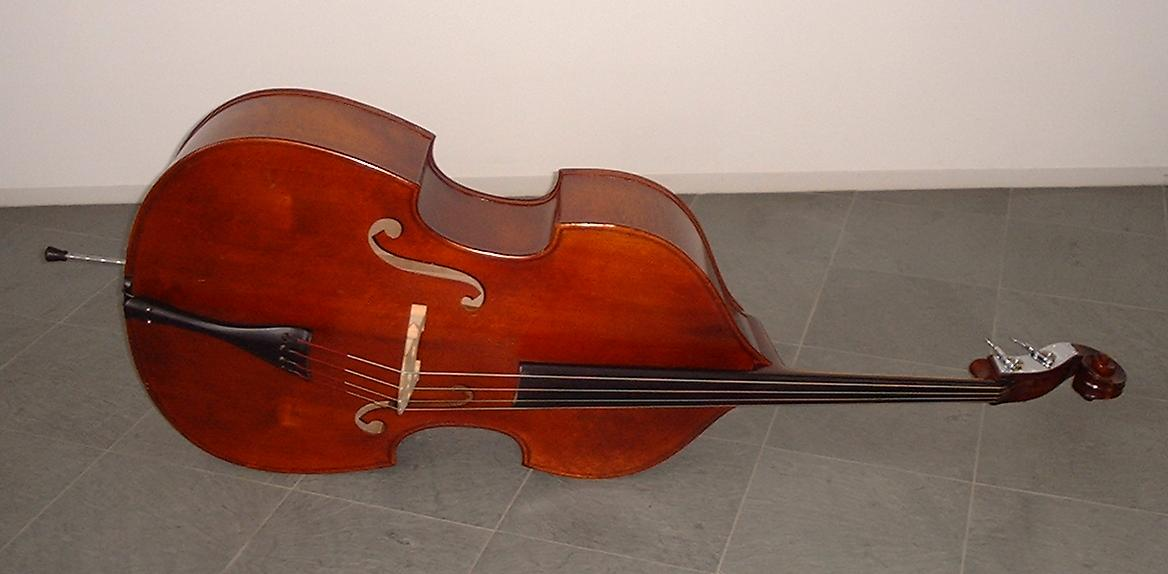
\includegraphics[height=2.7cm]{Pics/Instrument/on_earth.epsi}\\
{\small 図\thefigure : 床に置く場合\\}
\end{center}
\end{minipage}


\subsection{楽器の支え方}

図\addtocounter{figure}{1}\thefigure と図
\addtocounter{figure}{1}\thefigure の点線部分を対応させるようにして楽
器を体に当てます。\\
%ネックを持つ左手を除いて
%は、点線部分以外の部位で楽器に触れることはありません。\\

\addtocounter{figure}{-1}
\begin{minipage}{150pt}
\begin{center}
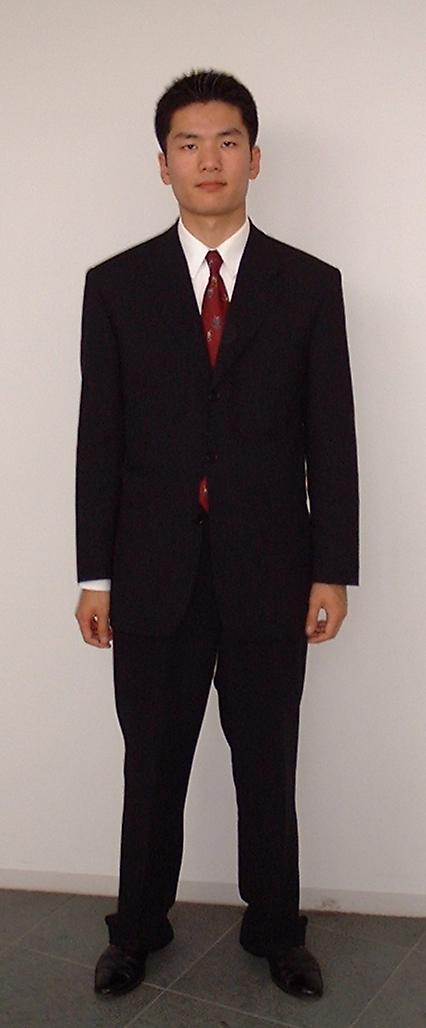
\includegraphics[height=7.35cm]{Pics/Instrument/standing.epsi}\\
{\small 図\thefigure : 足の付け根(点線部分)で支える\\}
\end{center}
\end{minipage}
\hfill
\begin{minipage}{110pt}
\begin{center}
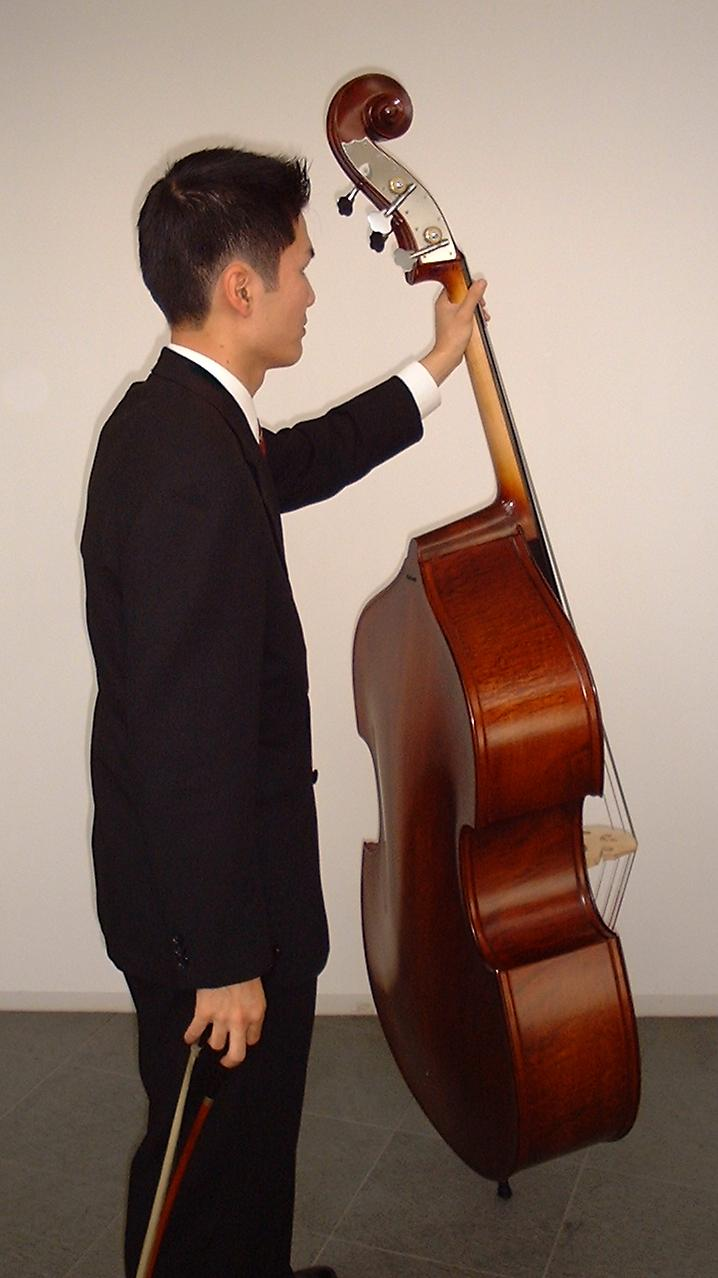
\includegraphics[height=7.35cm]{Pics/Instrument/edge.epsi}\\
\addtocounter{figure}{1}
{\small 図\thefigure : 点線は体に当てる部分\\}
\end{center}
\end{minipage}
\hfill
\begin{minipage}{140pt}
\begin{center}
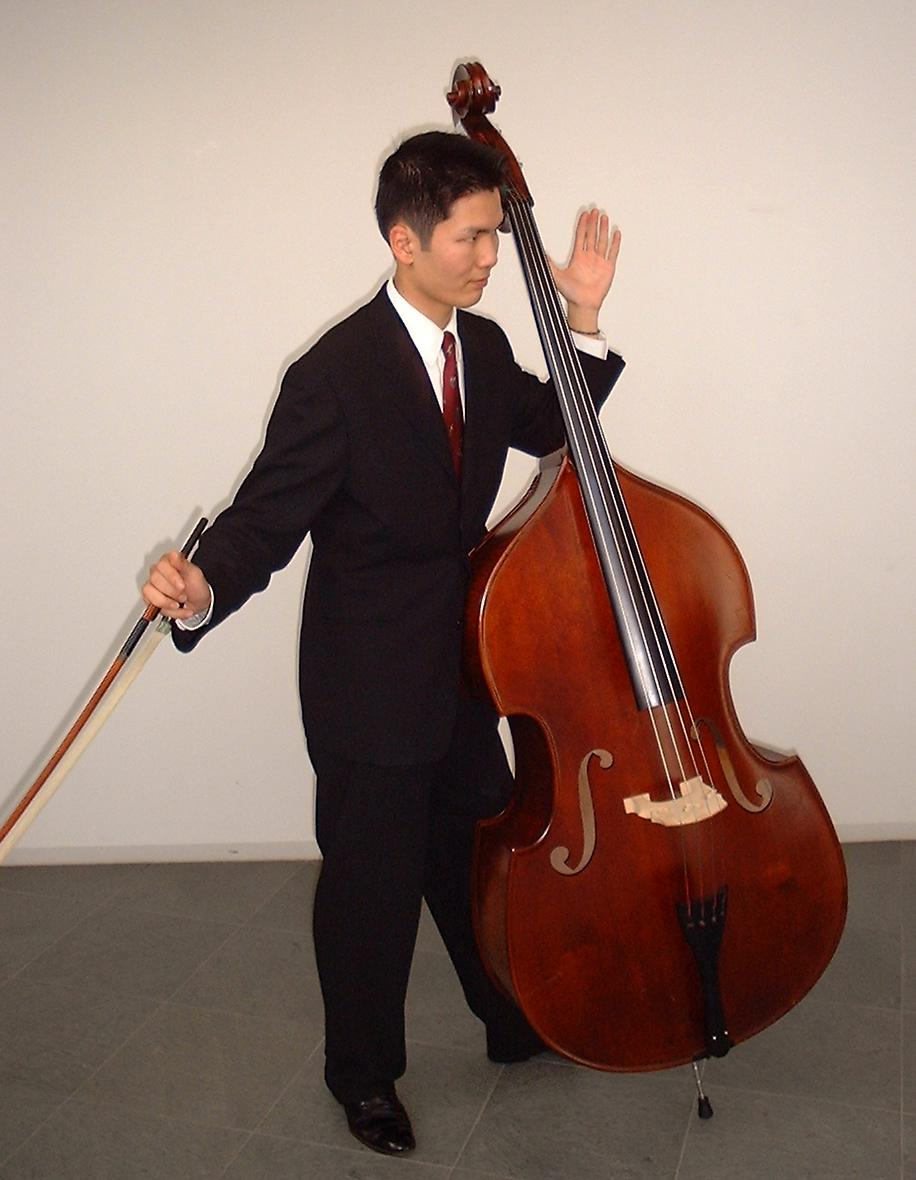
\includegraphics[height=7.35cm]{Pics/Instrument/without_hands.epsi}\\
\addtocounter{figure}{1}
{\small 図\thefigure : 手を触れずに支えるのが理想}
\end{center}
\end{minipage}

\ \\
\ \\


\begin{minipage}{190pt}
\ \ \ \ \addtocounter{figure}{-2}図\thefigure と図
\addtocounter{figure}{1}\thefigure の点線部分どうしをうまく対応させられない場合には、エンドピンの長さを調節して楽器の高さを合わせます。エンドピンとは楽器胴体の下端にネジで固定されている金属棒のことです。
\end{minipage}
\hfill
\begin{minipage}{220pt}
\begin{center}
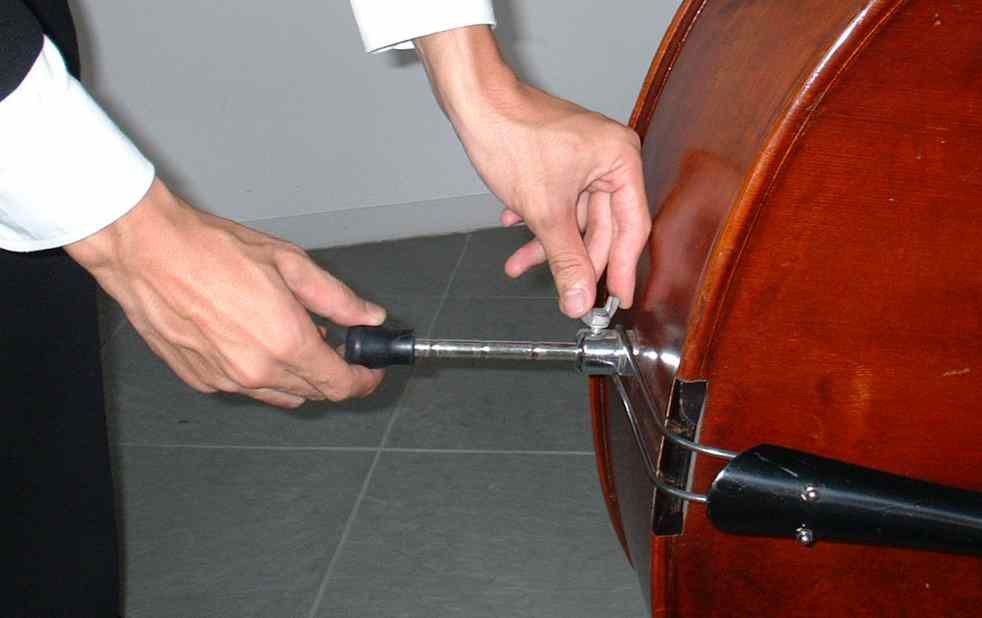
\includegraphics[height=3cm]{Pics/photo0830/endpin.epsi}\\
\addtocounter{figure}{2}
{\small 図\thefigure : ネジを緩めてエンドピンの長さを調節}
\end{center}
\end{minipage}

\ \\
\ \\

\begin{minipage}{120pt}
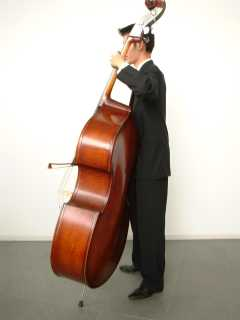
\includegraphics[height=7cm]{Pics/photo0830/stand_left.epsi}\\
\addtocounter{figure}{1}
{\small 図\thefigure : 楽器の支え方(左側から)}
\end{minipage}
\hfill
\begin{minipage}{120pt}
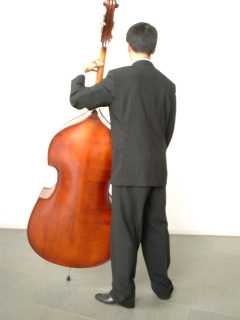
\includegraphics[height=7cm]{Pics/photo0830/stand_back.epsi}\\
\addtocounter{figure}{1}
{\small 図\thefigure : 楽器の支え方(背面から)}
\end{minipage}
\hfill
\begin{minipage}{120pt}
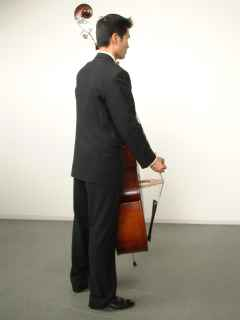
\includegraphics[height=7cm]{Pics/photo0830/stand_right.epsi}\\
\addtocounter{figure}{1}
{\small 図\thefigure : 楽器の支え方(右側から)}
\end{minipage}


\subsection{弓の毛}
弓の毛の張りは末端のネジで調節します。弾くときに張り、弾かないときは緩
めておきます。適度な弓の張りの目安は以下の2点を同時に満たすことです。

\begin{enumerate}
\item 弦に乗せて圧力をかけても竿が毛に触れない
\item 竿が反っている
\end{enumerate}

図\addtocounter{figure}{2}\thefigure のように竿に反りがない弓は明らか
に張りすぎです。弓の毛は消耗品ですので、1 年をめどに楽器店で交換しましょ
う。また、直接手で触れてはいけません。皮脂が付着して松ヤニの乗りが悪く
なります。\addtocounter{figure}{-1}
\begin{center}
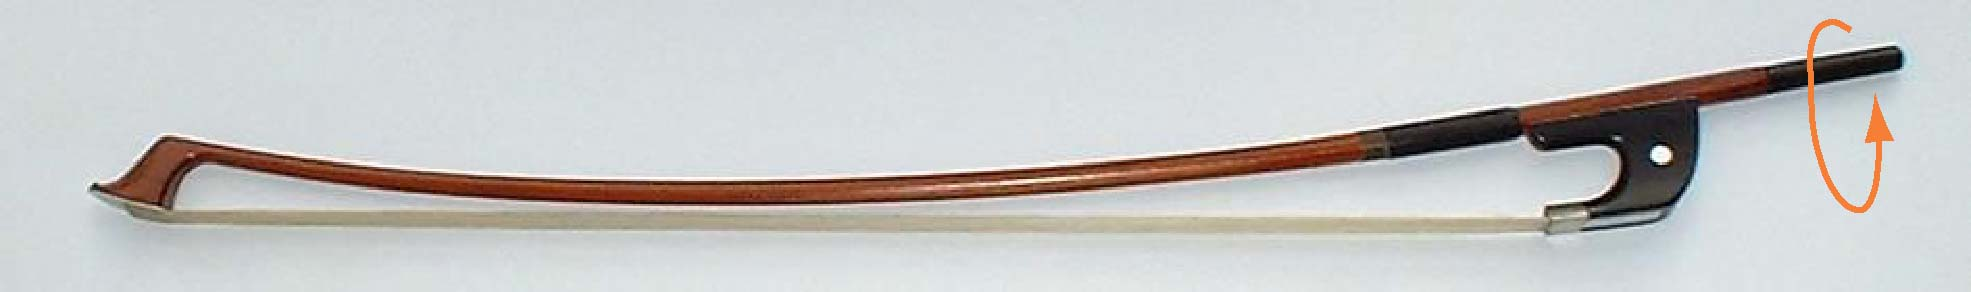
\includegraphics[width=13.5cm]{Pics/Bow/whole_bow_arrow.epsi}\\
{\small 図\thefigure : ネジを矢印の方向に回すと毛が緩む\\}
\end{center}
\addtocounter{figure}{1}
\begin{center}
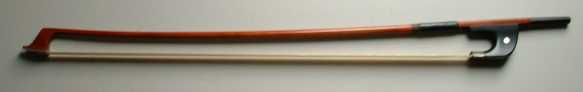
\includegraphics[width=13.5cm]{Pics/photo0830/tense_bow.epsi}\\
{\small 図\thefigure : 竿に反りがないのは張りすぎ\\}
\end{center}

\subsection{松ヤニ}
弓のすべり止めです。弓の毛と弦の間に松ヤニ粒子が介在して摩擦力が発生し
ます。弓毛を張ったら\addtocounter{figure}{2}図\thefigure のようにして
弓毛に塗付してください。また、練習終了後には弦に付着した松ヤニをタオル
で拭き取るようにしましょう\addtocounter{figure}{1}(図\thefigure )。\\
\indent 弦に付着した松ヤニと弓の松ヤニが異なると好ましくありません。な
るべくパート全員が同じ銘柄のものを使うようにしましょう。高温にさらすと
液化・変性してしまうので使用後はケースに入れて涼しい場所に保管します。

\begin{minipage}{180pt}
\addtocounter{figure}{-2}
\begin{center}
\includegraphics[height=3.5cm]{Pics/photo0830/rosin.epsi}\\
{\small 図\thefigure : 松ヤニとケース\\}
\end{center}
\end{minipage}
\hfill
\begin{minipage}{120pt}
\addtocounter{figure}{1}
\begin{center}
\includegraphics[height=3.5cm]{Pics/newphoto/rosin.epsi}\\
{\small 図\thefigure : 弓毛を張ったら塗る\\}
\end{center}
\end{minipage}
\hfill
\begin{minipage}{100pt}
\addtocounter{figure}{1}
\begin{center}
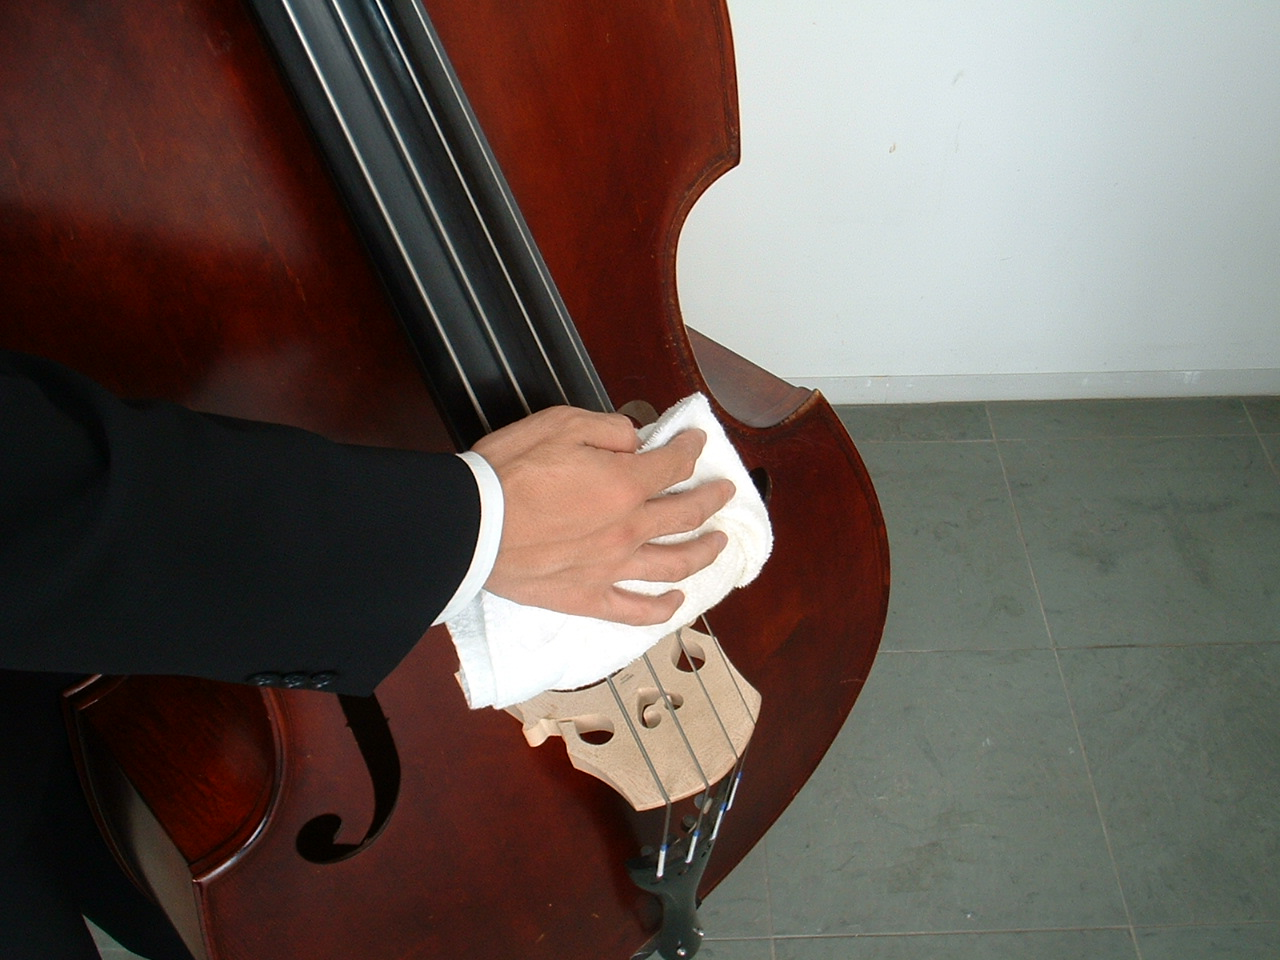
\includegraphics[height=3.5cm]{Pics/newphoto/towel.epsi}\\
{\small 図\thefigure : 練習後は拭き取る\\}
\end{center}
\end{minipage}

\subsection{弓の持ち方: (1) ドイツ式}
\underline{\bf 弓は主に親指と小指で持ちます}。図\addtocounter{figure}{1}\thefigure 〜図\addtocounter{figure}{3}\thefigure の順序に従って弓を持ってみましょう。\\

\begin{minipage}{200pt}
\begin{center}
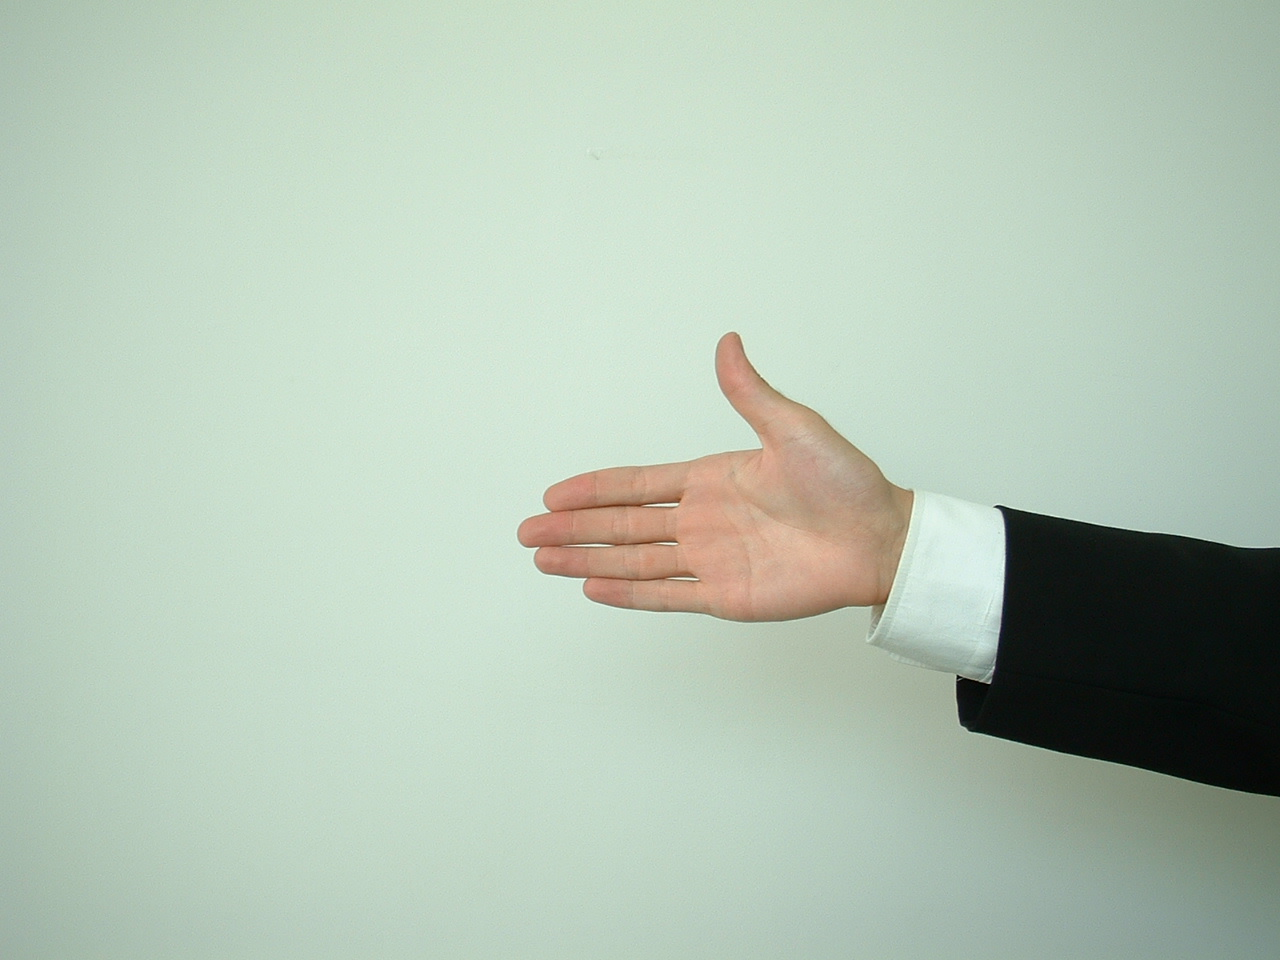
\includegraphics[height=4.3cm]{Pics/photo0830/righthand2.epsi}\\
\addtocounter{figure}{-3}
{\small 図\thefigure : 右手を構える\\}
\end{center}
\end{minipage}
\hfill
\begin{minipage}{200pt}
\begin{center}
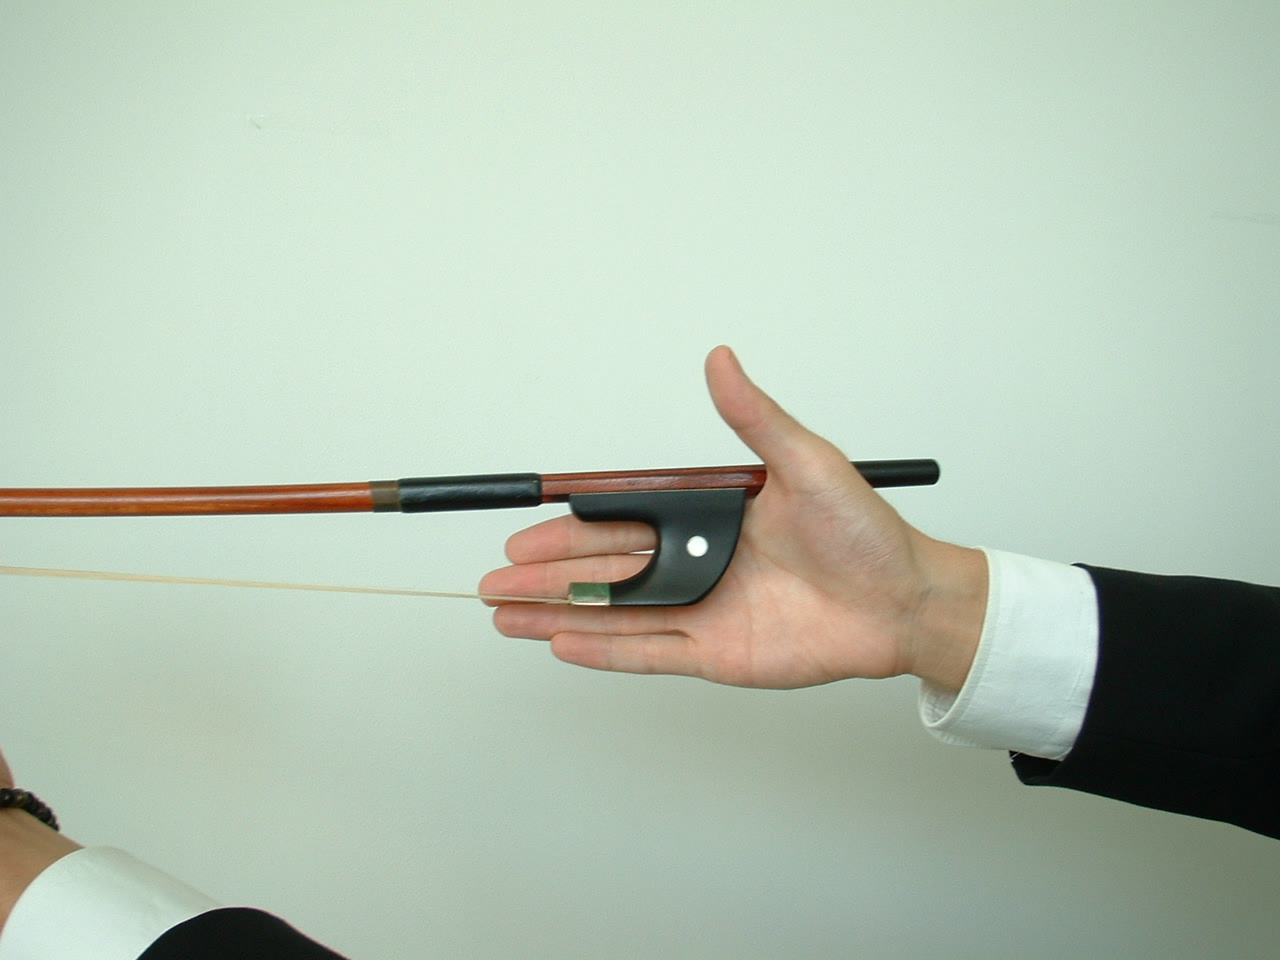
\includegraphics[height=4.3cm]{Pics/photo0830/righthand4.epsi}\\
\addtocounter{figure}{1}
{\small 図\thefigure : 弓の尾部を親指と人さし指の間に入れる\\}
\end{center}
\end{minipage}

\begin{minipage}{220pt}
\begin{center}
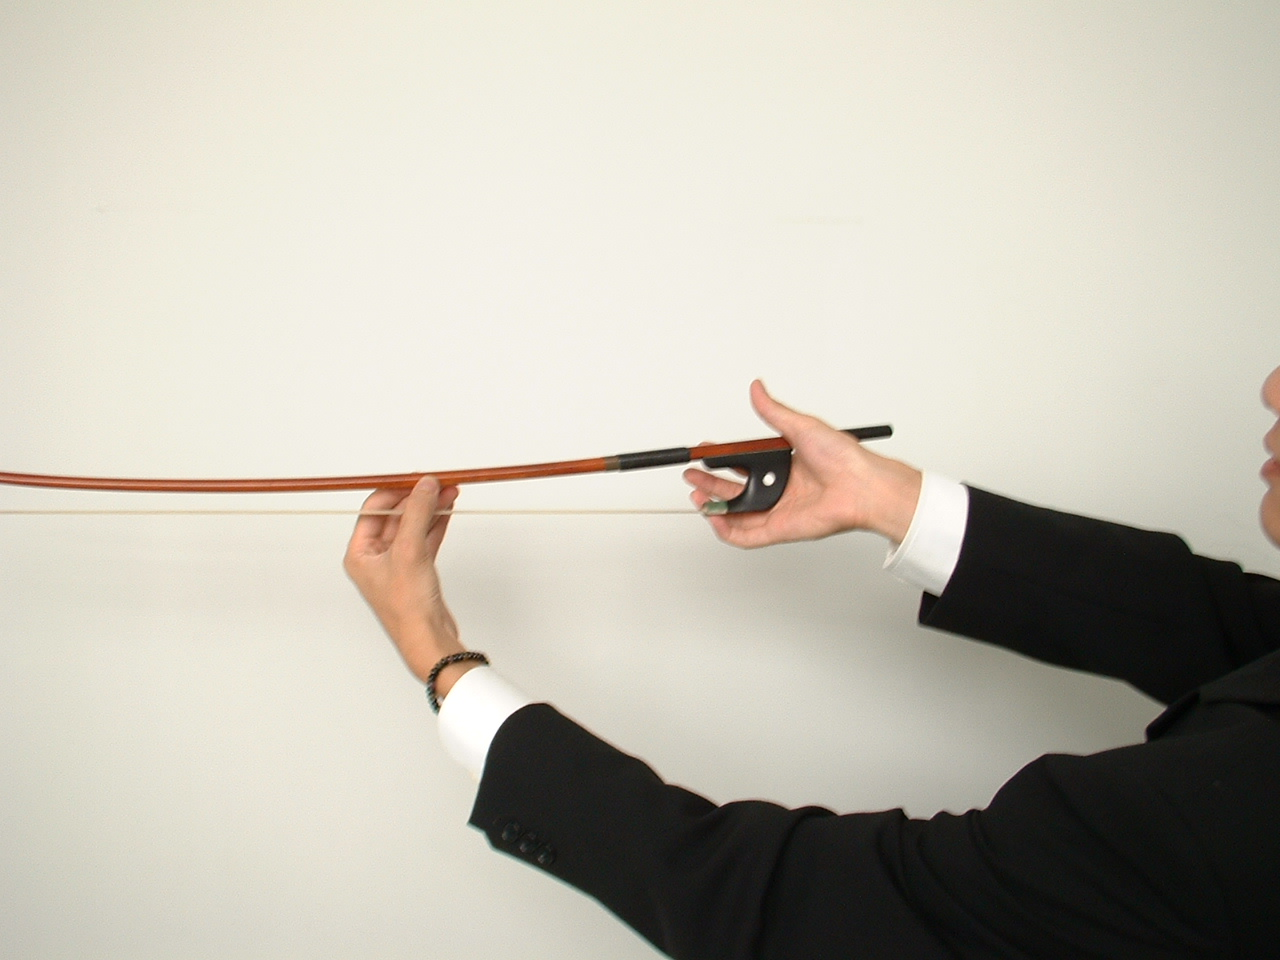
\includegraphics[height=4.3cm]{Pics/photo0830/bow3.epsi}\\
\addtocounter{figure}{1}
{\small 図\thefigure : 小指を丸めて金具を押さえる(図\addtocounter{figure}{2}\thefigure、図\addtocounter{figure}{1}\thefigure 参照)\\}
\end{center}
\end{minipage}
\hfill
\begin{minipage}{200pt}
\begin{center}
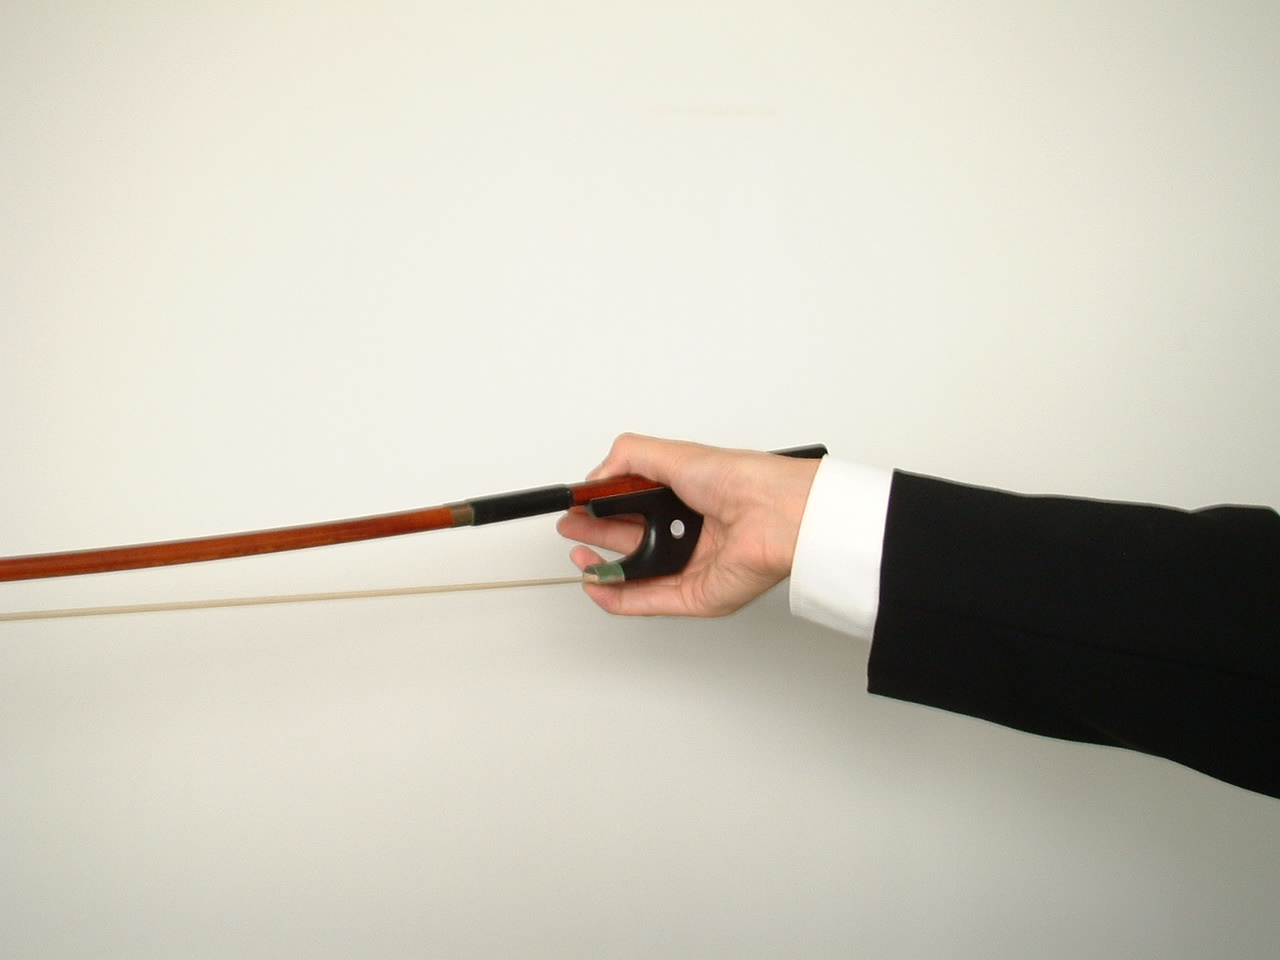
\includegraphics[height=4.3cm]{Pics/photo0830/bow4.epsi}\\
\addtocounter{figure}{-2}
{\small 図\thefigure : 親指を竿にかける(図\addtocounter{figure}{3}\thefigure〜\addtocounter{figure}{2}\thefigure 参照)\\}
\end{center}
\end{minipage}

\ \\

図\addtocounter{figure}{-6}\thefigure では小指を丸め、指先で弓毛の端にある金具を押さえます(図\addtocounter{figure}{2}\thefigure に網目で示した部分)。正しく押さえると図\addtocounter{figure}{1}\thefigure のようになります。また、図\addtocounter{figure}{-2}\thefigure において親指で竿を押さえる際には図\addtocounter{figure}{3}\thefigure 、\addtocounter{figure}{1}\thefigure に網目で示した部分どうしを重ね合わせ、図\addtocounter{figure}{1}\thefigure のようにします。\\

\begin{minipage}{120pt}
\addtocounter{figure}{-4}
\begin{center}
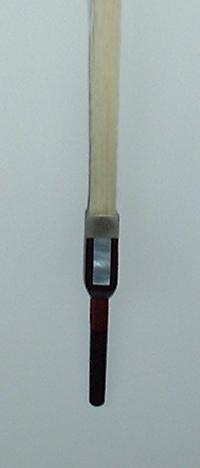
\includegraphics[height=8.8cm]{Pics/Bow/smallfinger_area.epsi}\\
{\small 図\thefigure : 小指が押さえる金具\\}
\end{center}
\end{minipage}
\hfill
\begin{minipage}{100pt}
\begin{center}
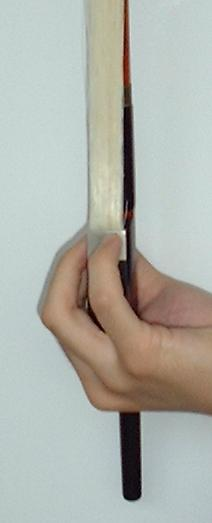
\includegraphics[height=8.8cm]{Pics/Bow/smallfinger.epsi}\\
\addtocounter{figure}{1}
{\small 図\thefigure : 小指\\}
\end{center}
\end{minipage}
\hfill
\begin{minipage}{110pt}
\addtocounter{figure}{1}
\begin{center}
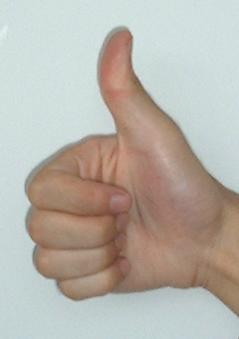
\includegraphics[width=2cm]{Pics/Bow/thumb.epsi}\\
{\small 図\thefigure : 親指と竿の接触部分(網目部分)\\}
\addtocounter{figure}{1}
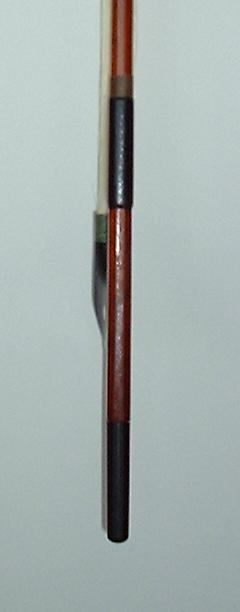
\includegraphics[width=2cm]{Pics/Bow/thumb_area.epsi}\\
{\small 図\thefigure : 親指と竿の接触部分(網目部分)\\}
\end{center}
\end{minipage}
\hfill
\begin{minipage}{80pt}
\addtocounter{figure}{1}
\begin{center}
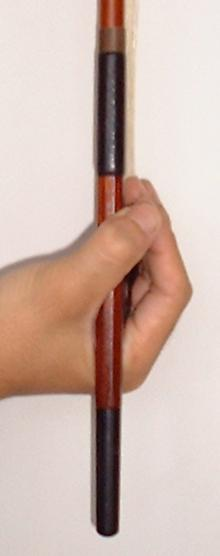
\includegraphics[height=8.8cm]{Pics/Bow/thumb_and_bow.epsi}\\
{\small 図\thefigure : 親指と竿\\}
\end{center}
\end{minipage}

以上の手続きに従って正しく弓を持てたときの手の形を図
\addtocounter{figure}{1}\thefigure 〜図
\addtocounter{figure}{2}\thefigure に示しました。なお、初心者にありが
ちな間違いとして図\addtocounter{figure}{1}\thefigure のように竿と弓毛
の間に人さし指、中指、薬指のいずれかを入れることが見られますが、これは
手首の柔軟な動きを損なうので避けましょう。\\\underline{\bf 親指・小指以
外の中3本の指は軽く添えるだけです}。\\

\begin{minipage}{210pt}
\addtocounter{figure}{-3}
\begin{center}
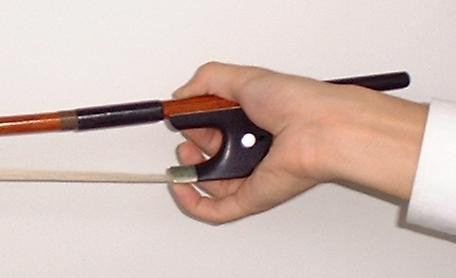
\includegraphics[height=4.3cm]{Pics/Bow/perspective_1.epsi}\\
{\small 図\thefigure : 弓の持ち方(手の平側)}
\end{center}
\end{minipage}
\hfill
\begin{minipage}{210pt}
\addtocounter{figure}{1}
\begin{center}
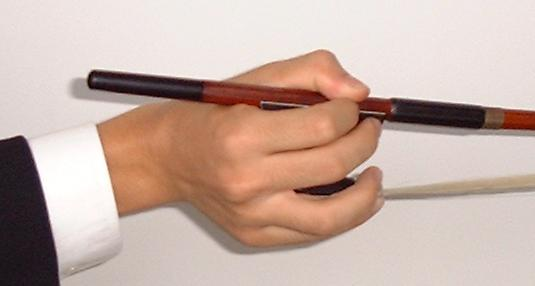
\includegraphics[height=4.3cm]{Pics/Bow/perspective_2.epsi}\\
{\small 図\thefigure : 弓の持ち方(手の甲側)}
\end{center}
\end{minipage}

\begin{minipage}{200pt}
\begin{center}
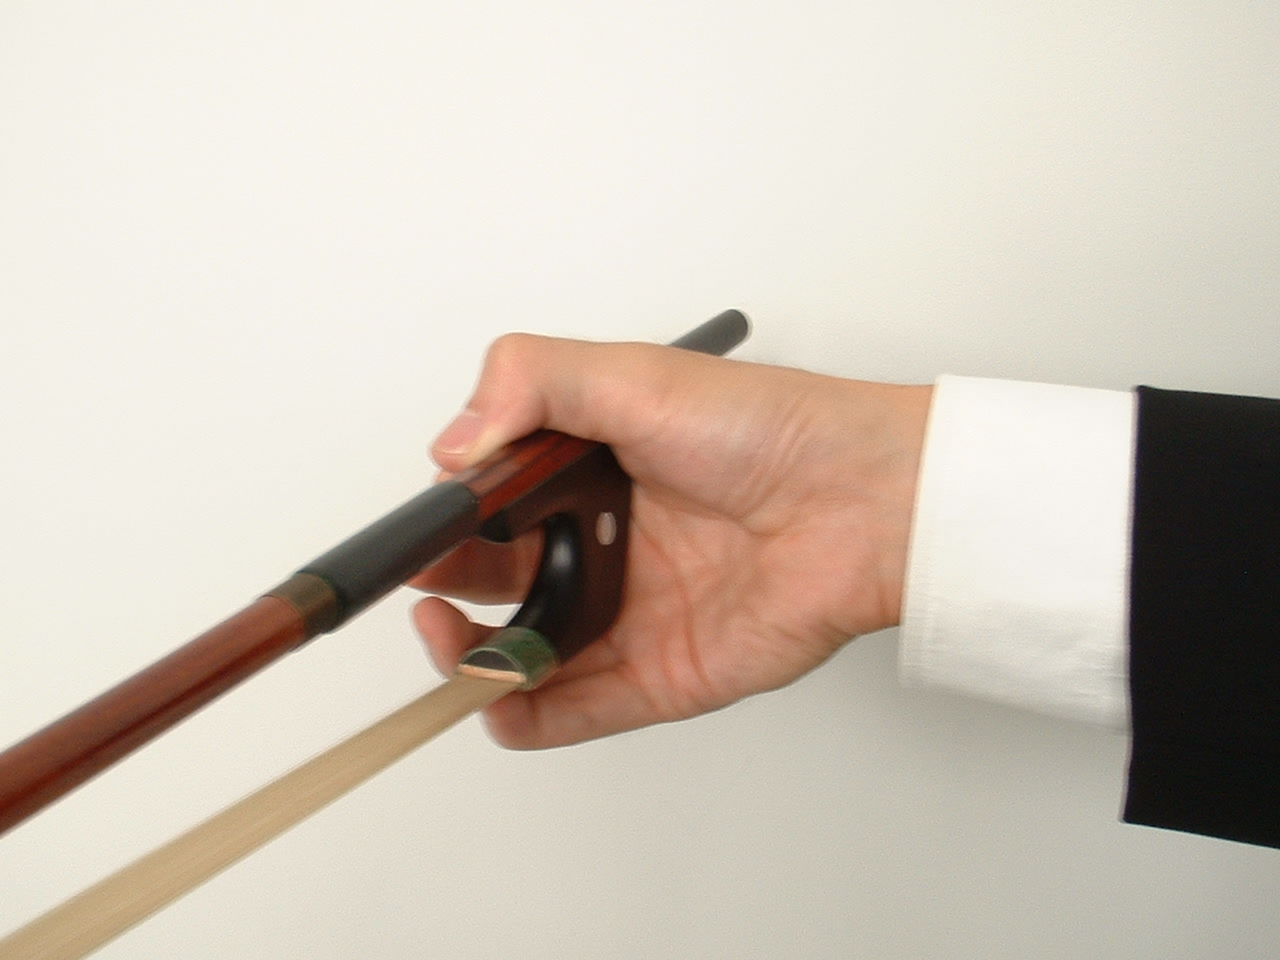
\includegraphics[height=4.3cm]{Pics/photo0830/bow5.epsi}\\
\addtocounter{figure}{1}
{\small 図\thefigure : 手の平は毛箱を包み込むように\\}
\end{center}
\end{minipage}
\hfill
\begin{minipage}{200pt}
\begin{center}
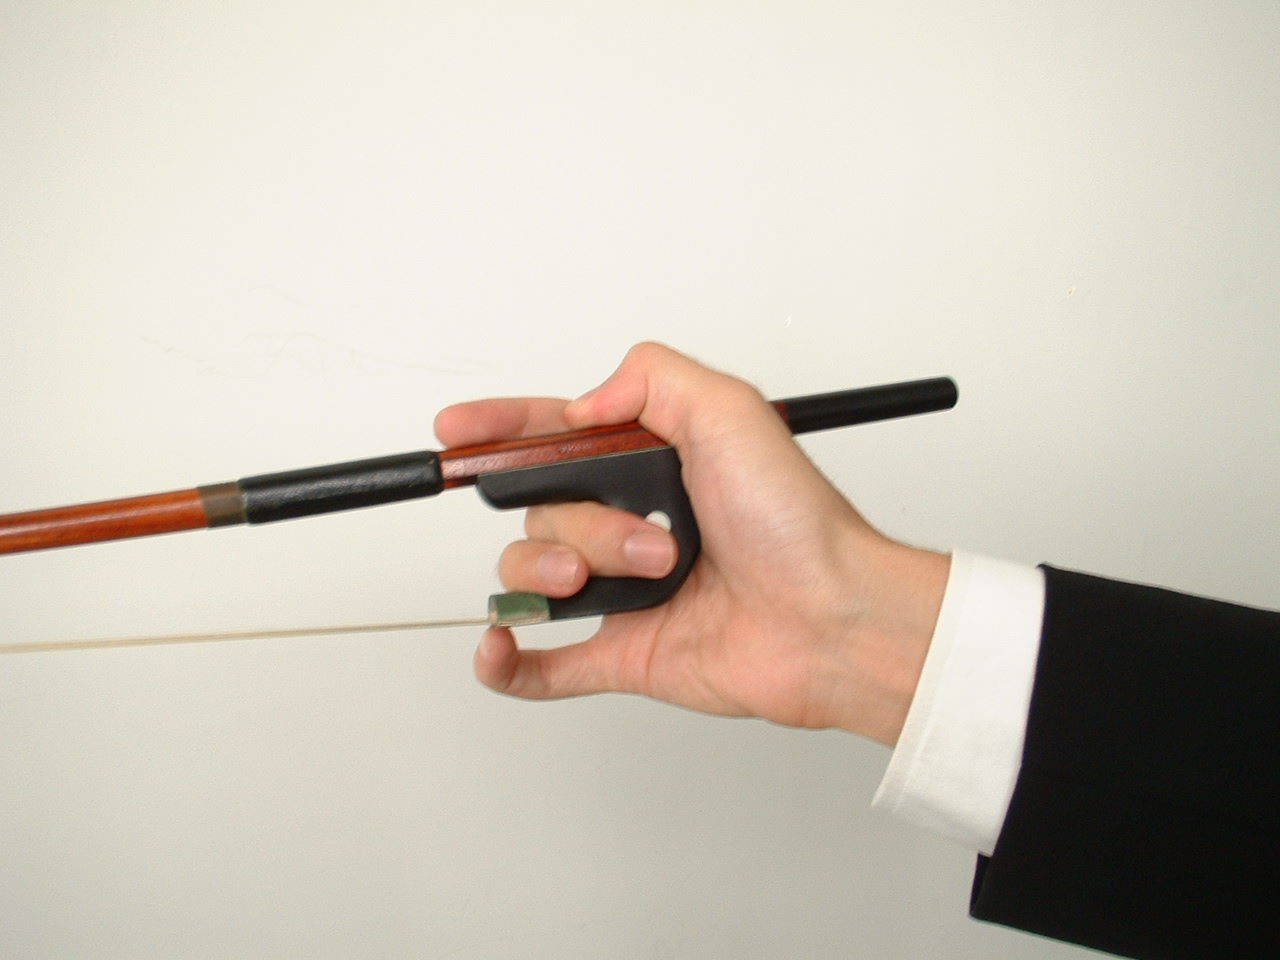
\includegraphics[height=4.3cm]{Pics/photo0830/badbow.epsi}\\
\addtocounter{figure}{1}
{\small 図\thefigure : 悪い例(竿と弓毛の間に指を入れない)\\}
\end{center}
\end{minipage}

\subsection{弓の持ち方: (2) フランス式}



\subsection{弓で弦を弾く}
弓は\ruby{指}{し}\ruby{板}{ばん}の端から駒までの間に置きます(図
\addtocounter{figure}{1}\thefigure)。弓の軌道が弦に対して垂直に交差す
るように動かします(図\addtocounter{figure}{1}\thefigure)。鏡を利用して
弓の軌道を確認しながら練習するのも有効でしょう。どの弦でもいいので、以
下の順序に従って音を鳴らしてみましょう。

\begin{flushleft}
\begin{minipage}{200pt}

\begin{enumerate}
\item 竿を指板側に少し傾ける(図\addtocounter{figure}{1}\thefigure 、\addtocounter{figure}{1}\thefigure) 
\item 親指に力を入れて弦に圧力をかける
\item 弓を動かす
\item 音が鳴りだしたら親指の力を抜く。弓は動かし続ける。
\end{enumerate}
\end{minipage}
\hfill
\begin{minipage}{110pt}
\begin{center}
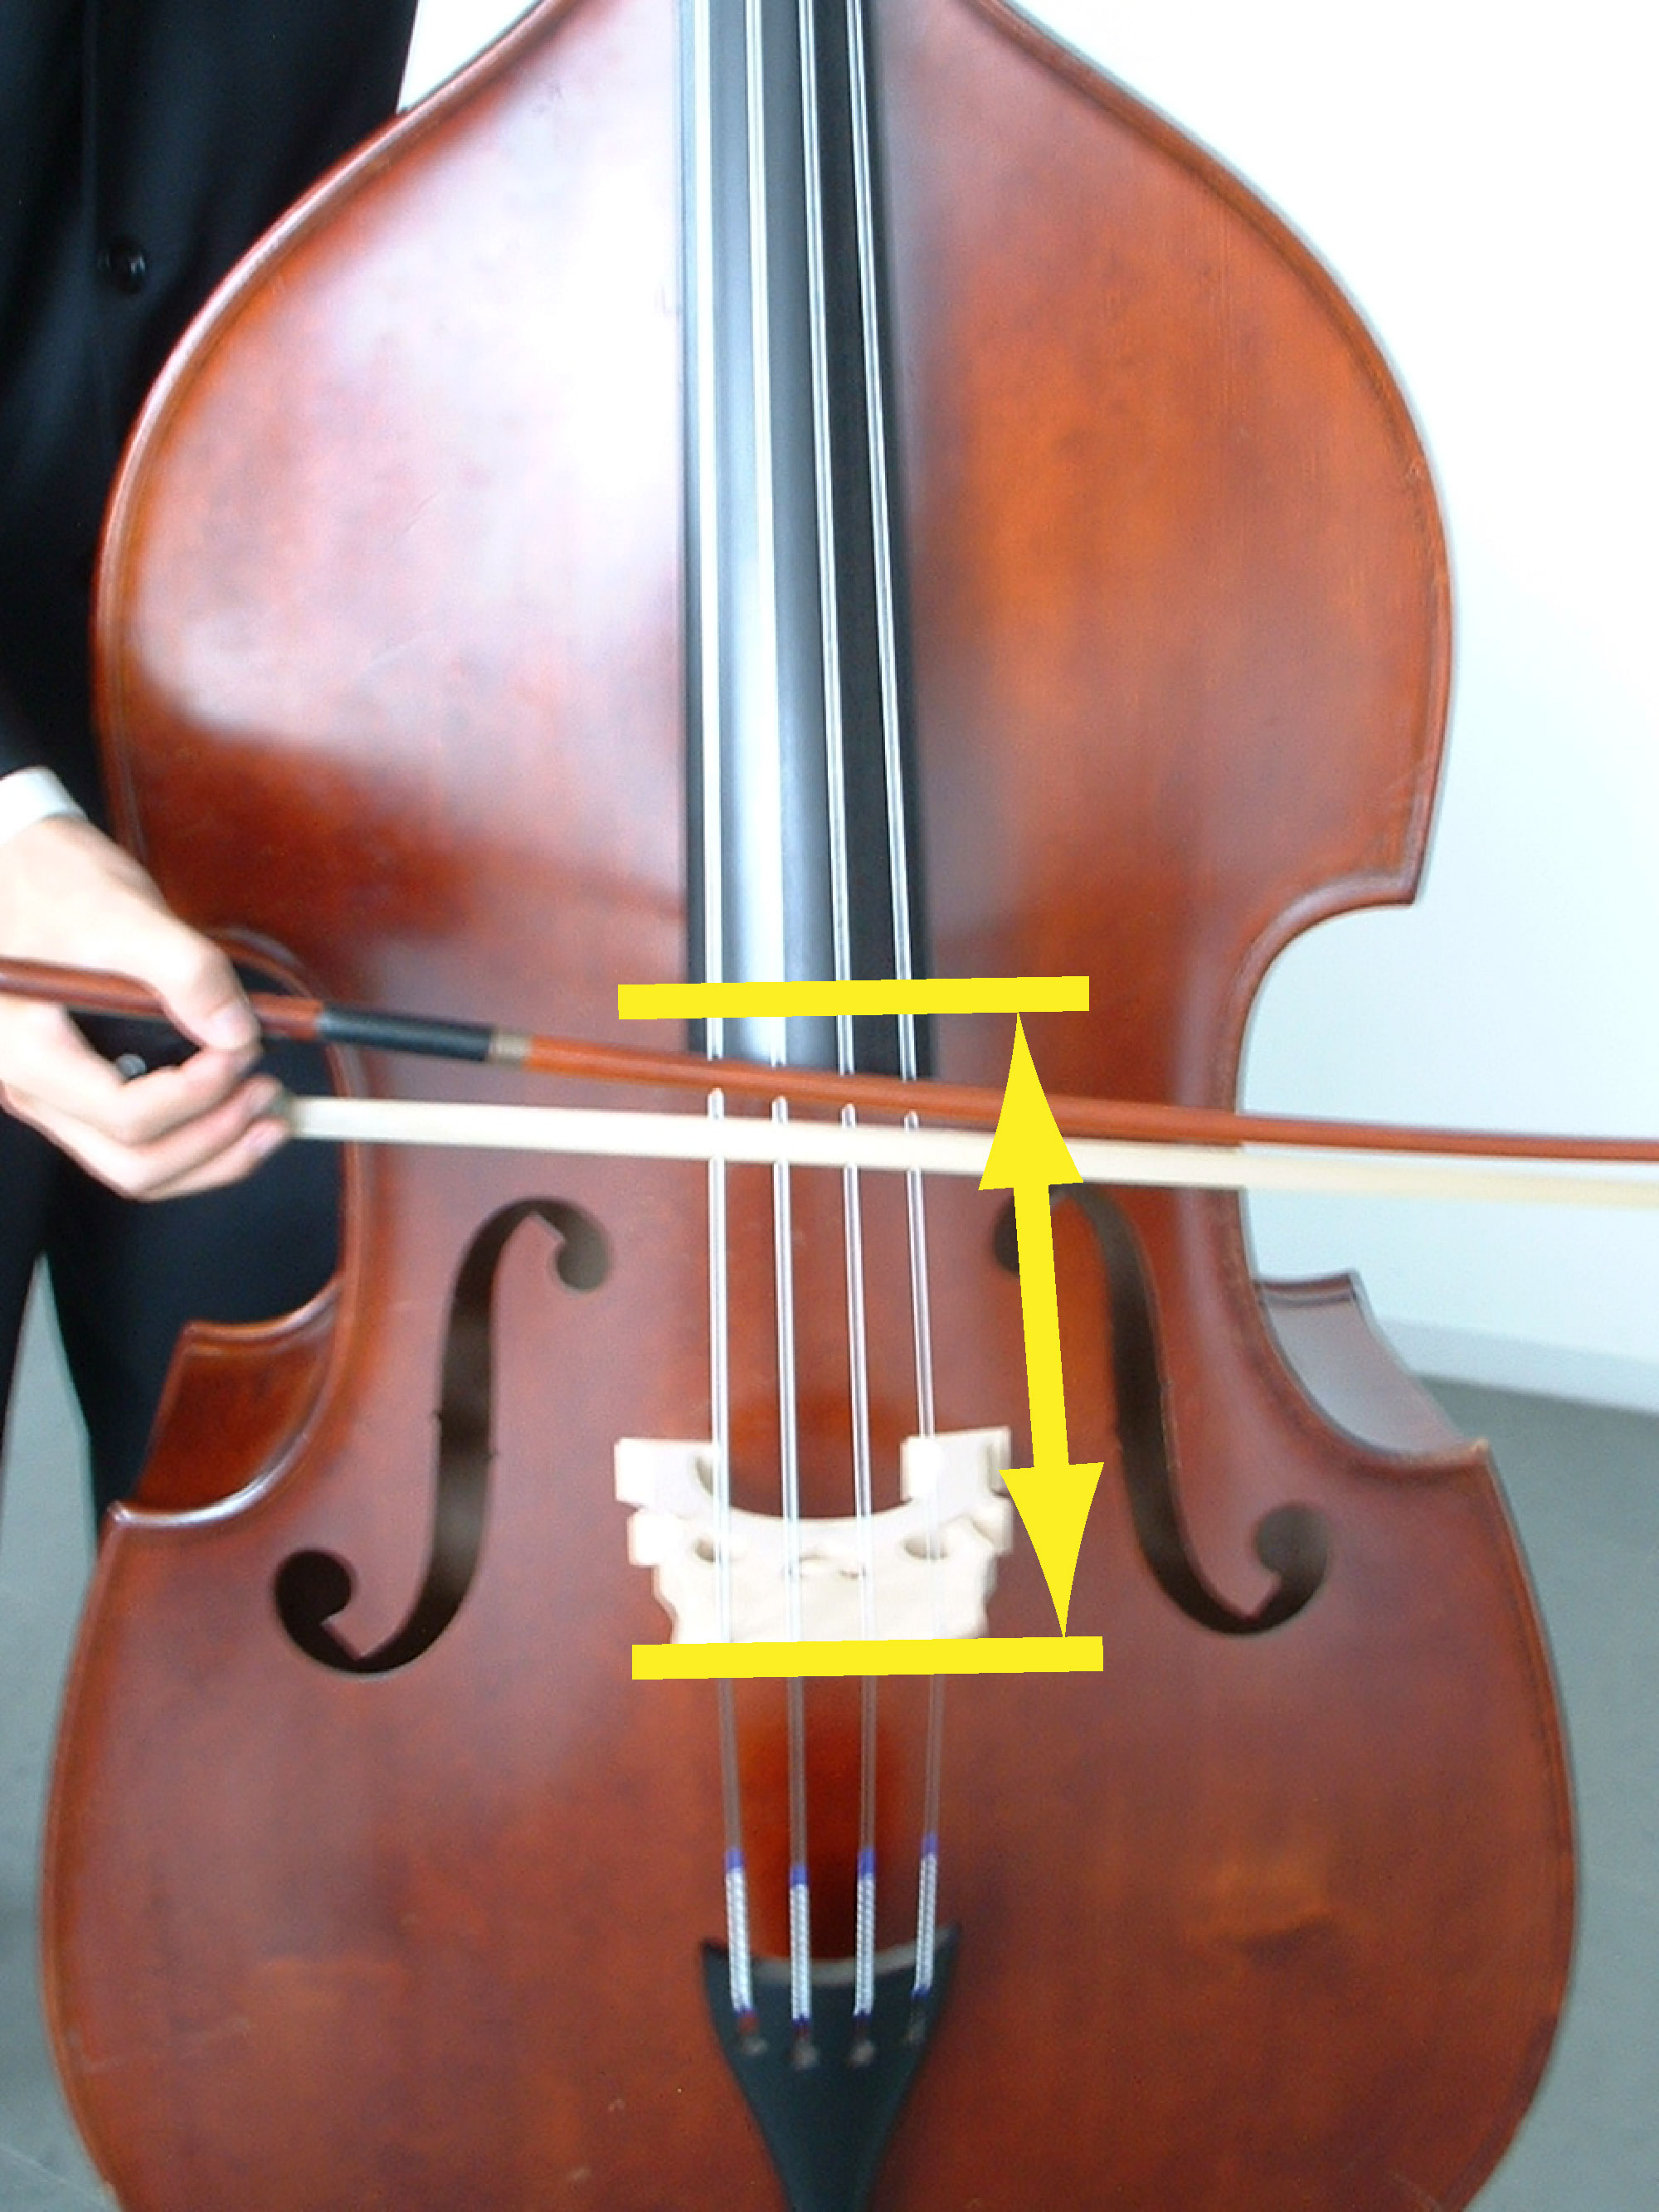
\includegraphics[height=3.4cm]{Pics/photo0830/bowbass2.epsi}\\
\addtocounter{figure}{-3}
{\small 図\thefigure : 矢印の範囲内を弾く\\}
\end{center}
\end{minipage}
\hfill
\begin{minipage}{110pt}
\begin{center}
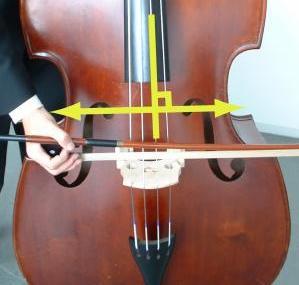
\includegraphics[height=3.4cm]{Pics/photo0830/bowbass1.epsi}\\
\addtocounter{figure}{1}
{\small 図\thefigure : 弓の軌道は弦と直交\\}
\end{center}
\end{minipage}

\begin{minipage}{205pt}
\ \ \ \ 親指の力がうまく弦に伝わると、振幅がはっきりと見えるほど弦が振
動します。一旦振動が始まったら、親指から力を抜きます。あとは弓を動かし
ているだけで振動を保つことができます。\\
\end{minipage}
\hfill
\begin{minipage}{110pt}
\begin{center}
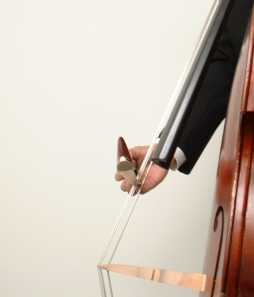
\includegraphics[height=4cm]{Pics/photo0830/bow_string1.epsi}\\
\addtocounter{figure}{1}
{\small 図\thefigure : 竿を指板側に傾ける\\}
\end{center}
\end{minipage}
\hfill
\begin{minipage}{110pt}
\begin{center}
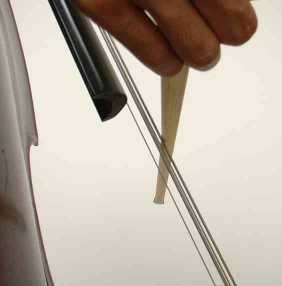
\includegraphics[height=4cm]{Pics/photo0830/bow_string2.epsi}\\
\addtocounter{figure}{1}
{\small 図\thefigure : 右側から見た図\\}
\end{center}
\end{minipage}
\end{flushleft}

\clearpage

\subsection{音量}
大まかに言って、音量は以下の4要素の組合せで決まります。\\

\begin{quote}
\begin{enumerate}
\item 右手親指の圧力\  (強いほど音量大)
\item 駒からの距離\ \ \ \  (駒に近いほど音量大)
\item 弓先か弓元か\ \ \ \ (弓の先ほど繊細な音を出しやすい)
\item 弓を動かす速さ\  (速ければ力強い音、ゆっくりなら柔和な音)
\end{enumerate}
\end{quote}

音量や音色は奥が深いテーマですので、本書ではこれ以上立ち入らないことにします。

\subsection{開放弦}
左手で弦を押さえていない状態のことを\underline{\bf 開放弦}と呼びます。コントラバスの開放弦は太い方から順にE\(\longrightarrow\)A\(\longrightarrow\)D\(\longrightarrow\)Gというよ
うに4度ずつ上がっていきます\footnote{ヴィオラ、チェロはヴァイオリンを原型とする「ヴァイオリン属」に含まれ、太い弦から順に5度ずつ上がる。一方、コントラバスは前3者とは異なりヴィオールという楽器を原型とする「ヴィオール属」である。調弦の違いはここに由来する。}。

\begin{music}
\nostartrule
\parindent 0pt
\setclef1{\bass}  
\startextract
\Notes\zchar{-7}{\ \ \ \ \ E}\enotes
\NOTEs\wh{E}\enotes
\doublebar
\Notes\zchar{-7}{\ \ \ \ \ A}\enotes
\NOTEs\wh{'A}\enotes
\doublebar
\Notes\zchar{-7}{\ \ \ \ \ D}\enotes
\NOTEs\wh{'D}\enotes
\doublebar
\Notes\zchar{-7}{\ \ \ \ \ G}\enotes
\NOTEs\wh{'G}\enotes
\setdoublebar
\endextract
\end{music}


なお、記譜上の慣習として、コントラバスの譜面は実音よりも1オクターヴ上に書かれます。逆に言えば、楽譜に書かれた音を弾くと、コントラバスはその1オクターヴ下の音を出します。

\subsection{チューニングメーター}
\begin{flushleft}
\begin{minipage}{320pt}
\ \ \ \ \ 音程を合わせる装置です。練習を始める前には必ずチューニングメー
ターを用いて開放弦の音程を合わせておきましょう。
\addtocounter{figure}{3}図\thefigure のようにしてコンタクトマイクを通
して集音すれば、うるさい場所でも確実に自分の楽器の音を拾ってくれます。
\\

\begin{minipage}{150pt}
\addtocounter{figure}{-2}
\begin{center}
\includegraphics[width=3cm]{Pics/newphoto/tuner.epsi}\\
{\small 図\thefigure : チューニングメーター\\}
\end{center}
\end{minipage}
\hfill
\begin{minipage}{150pt}
\addtocounter{figure}{1}
\begin{center}
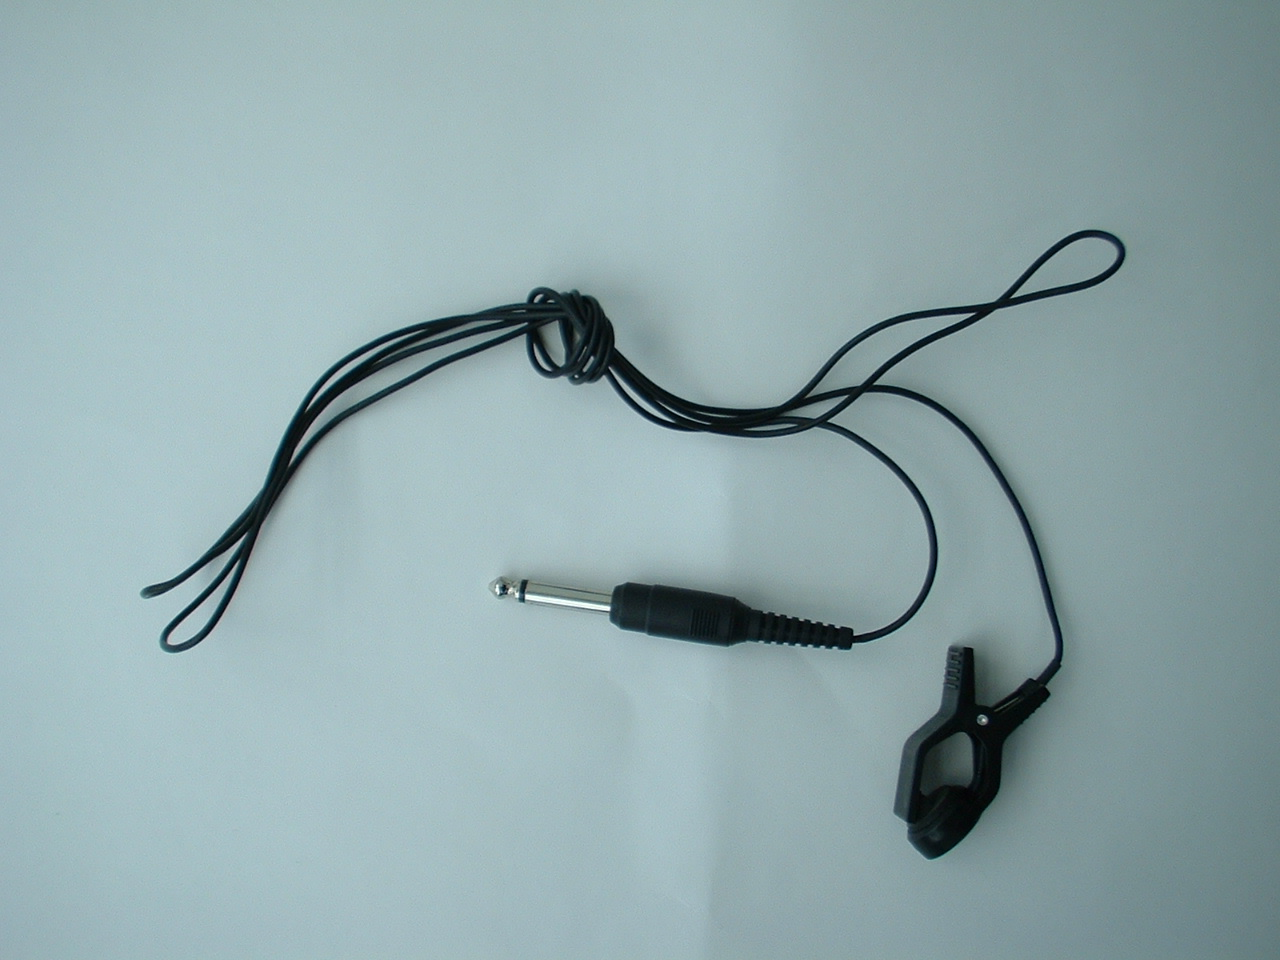
\includegraphics[width=2.7cm]{Pics/newphoto/contact1.epsi}\\
{\small 図\thefigure : コンタクトマイク\\}
\end{center}
\end{minipage}
\end{minipage}
\hfill
\begin{minipage}{110pt}
\addtocounter{figure}{1}
\begin{center}
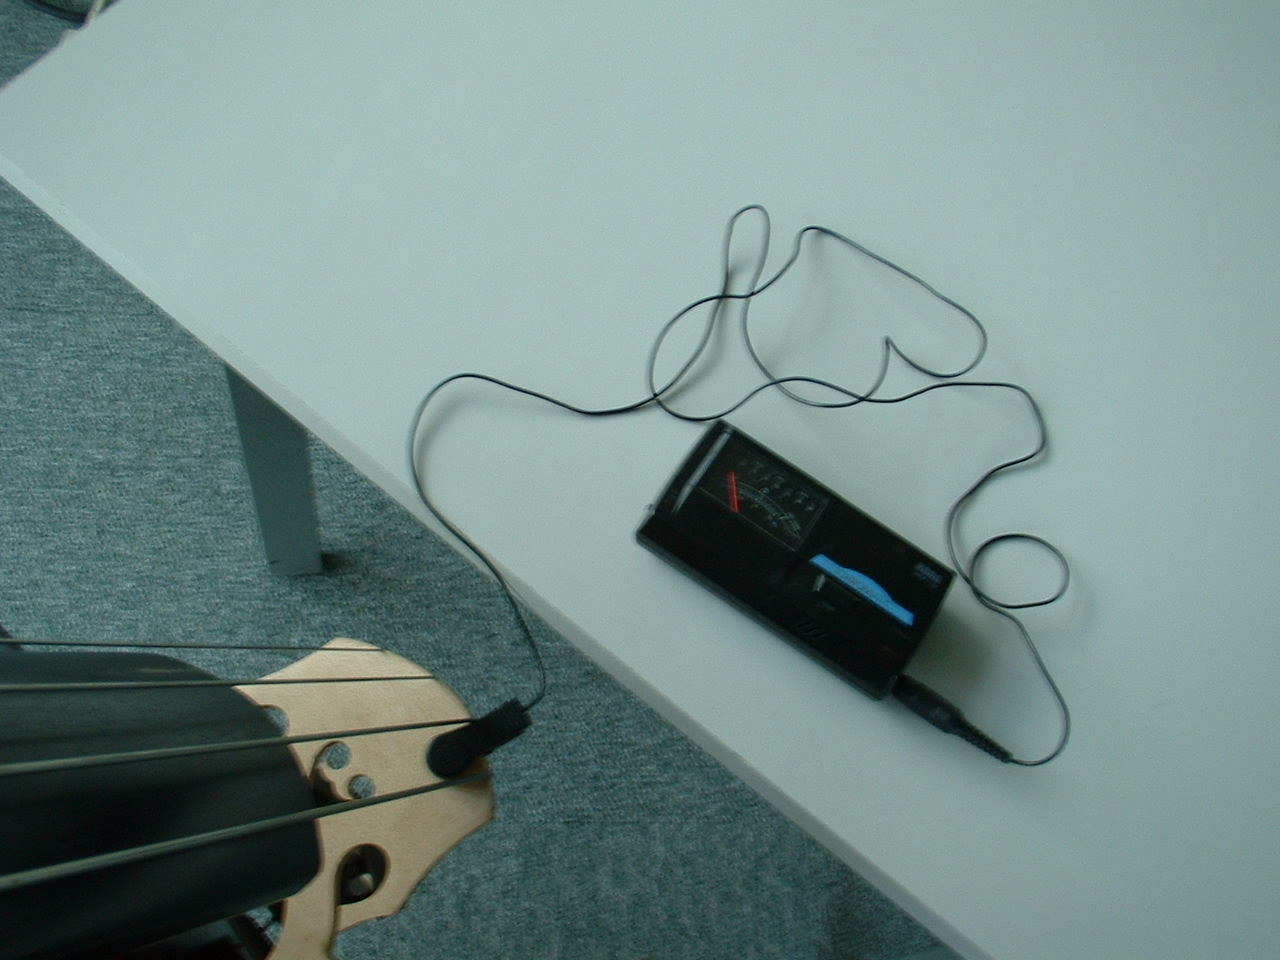
\includegraphics[width=4cm]{Pics/newphoto/contact2.epsi}\\
{\small 図\thefigure : マイクを駒にはさむ\\}
\end{center}
\end{minipage}
\end{flushleft}

\subsection{ボウイング(英: bowing)の記号}
\addtocounter{figure}{1}
\begin{center}
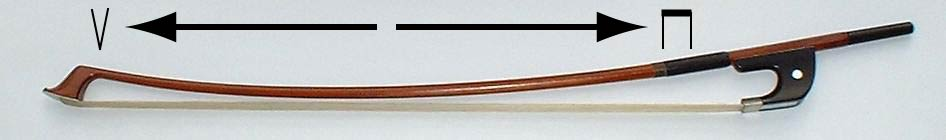
\includegraphics[width=12.5cm]{Pics/Bow/updown_bow.epsi}\\
{\small 図\thefigure : ボウイング記号とその示す方向\\}
\end{center}

\begin{center}
\begin{music}
\downbow 
\end{music}
\ \ \ \(\cdots\) ダウン・ボウ(通称「ダウン」)。弓を手元の方向へ動かします。

\begin{music}
\upbow 
\end{music}
\ \ \ \(\cdots\) アップ・ボウ(通称「アップ」)。弓を弓先の方向へ動かします。
\end{center}

小節の頭など強拍のところはダウン・ボウで弾く場合が多数です。逆に弱拍の音符はアップ・ボウで弾くのが一般的です。

\subsection{開放弦の練習 \label{open1}}
\begin{flushleft}
\begin{minipage}{310pt}
\ \ \ \ 調弦が終わったら、下の譜例\cite[pp.7]{simandl}を用いて開放弦で
音を鳴らす練習をしてみましょう。\underline{\bf 音量が均一になるように} 
気を配って下さい。また、今後はどんな練習をするときにも必ずメトロノーム
を使いましょう。オーケストラにおいてコントラバスは打楽器に次ぐ重要なリ
ズム楽器ですので、日頃からリズム感を磨いておきます。電子音でリズムを示
すものよりも打撃音でリズムを教えてくれるぜんまい式メトロノームの方が音
の通りが良く使いやすいでしょう。\\
\end{minipage}
\hfill
\begin{minipage}{120pt}
\addtocounter{figure}{1}
\begin{center}
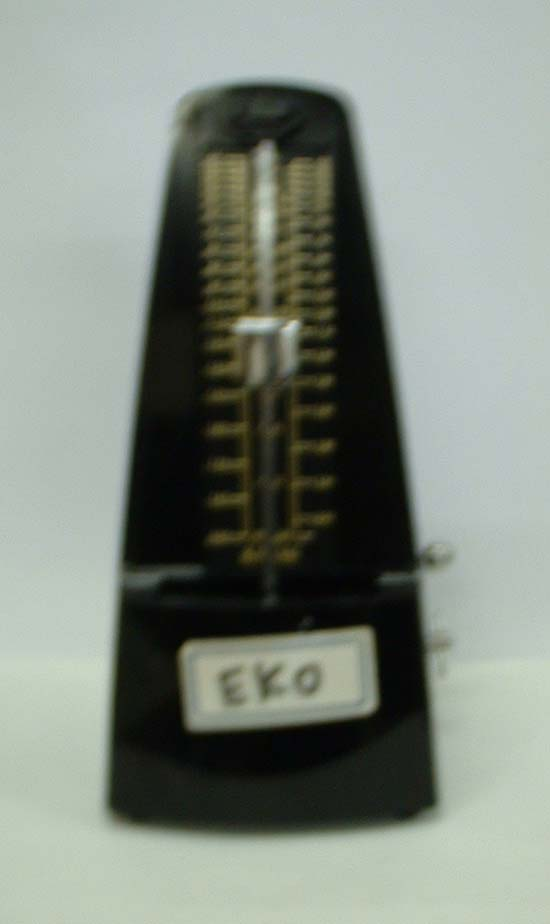
\includegraphics[height=4cm]{Pics/newphoto/metronome.epsi}\\
{\small 図\thefigure : ぜんまい式メトロノーム\\}
\end{center}
\end{minipage}
\end{flushleft}

\begin{music}
\nostartrule
\parindent 0pt
\setclef1{\bass}  
\generalmeter{\meterC}
\startpiece
\notes\zchar{14}{(\metron{\qu}{60})}\enotes
\NOtes\zchar{9}{\downbow}\wh{'D}\enotes
\bar
\notes\enotes
\NOtes\zchar{9}{\upbow}\wh{'A}\enotes
\bar
\notes\enotes
\NOtes\wh{'D}\enotes
\bar
\notes\enotes
\NOtes\wh{'G}\enotes
\bar
\notes\enotes
\NOtes\wh{'A}\enotes
\bar
\notes\enotes
\NOtes\wh{'D}\enotes
\bar
\notes\enotes
\NOtes\wh{E}\enotes
\bar
\notes\enotes
\NOtes\wh{'A}\enotes
\endpiece

\startpiece
\notes\enotes
\Notes\zchar{9}{\downbow}\hl{'D}\zchar{9}{\upbow}\hl{D}\enotes
\bar
\Notes\hu{'A}\hu{A}\enotes
\bar
\Notes\hl{'D}\hl{D}\enotes
\bar
\Notes\hl{'G}\hl{G}\enotes
\bar
\Notes\hu{'A}\hu{A}\enotes
\bar
\Notes\hl{'D}\hl{D}\enotes
\bar
\Notes\hu{E}\hu{E}\enotes
\bar
\Notes\hu{'A}\hu{A}\enotes
\endpiece

\startpiece
\notes\zchar{9}{\downbow}\ql{'D}\zchar{9}{\upbow}\ql{DDD}\enotes
\bar
\notes\qu{'AAAA}\enotes
\bar
\notes\ql{'DDDD}\enotes
\bar
\notes\ql{'GGGG}\enotes
\bar
\notes\qu{'AAAA}\enotes
\bar
\notes\ql{'DDDD}\enotes
\bar
\notes\qu{EEEE}\enotes
\bar
\notes\qu{'AAAA}\enotes
\rightrepeat
\Notes\wh{'D}\enotes
\setdoublebar
\endpiece
\end{music}

\subsection{移弦 \label{strchg}}

\begin{minipage}{230pt}
\ \ \ \ 「\ref{open1}」の開放弦の練習をしてみて、音符と音符との間に音
が鳴っていない時間ができてしまいませんでしたか? もしそうなら、その理由
の1つは弦から弦への弓の移動(移弦)が滑らかでないことです。図
\addtocounter{figure}{1}\thefigure は、D線を弾いている弓の軌道を、徐々
に移動先のA線に近い軌道に移す様子を示しています。図中の数字は以下の弓
の軌道に対応します。

\begin{enumerate}
\item D線を弾く際の基本的な軌道
\item D線を弾きながらA線にぎりぎりまで近付く
\item A線に移った直後の軌道。この状態からA線を弾き始める。
\item A線を弾く際の基本的な軌道に移る
\end{enumerate}

図\addtocounter{figure}{1}\thefigure 、図\addtocounter{figure}{1}\thefigure は移弦の際の右手の動きを示しています。\\
\end{minipage}
\hfill
\begin{minipage}{180pt}
\begin{center}
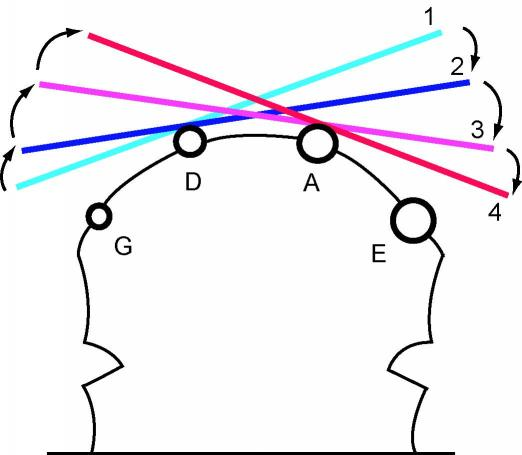
\includegraphics[height=5cm]{Pics/photo0830/strchg6.epsi}\\
\addtocounter{figure}{-2}
{\small 図\thefigure : D線からA線への移弦(1\(\rightarrow\)2\(\rightarrow\)3\(\rightarrow\)4)\\}
\end{center}
\end{minipage}

\begin{minipage}{200pt}
\begin{center}
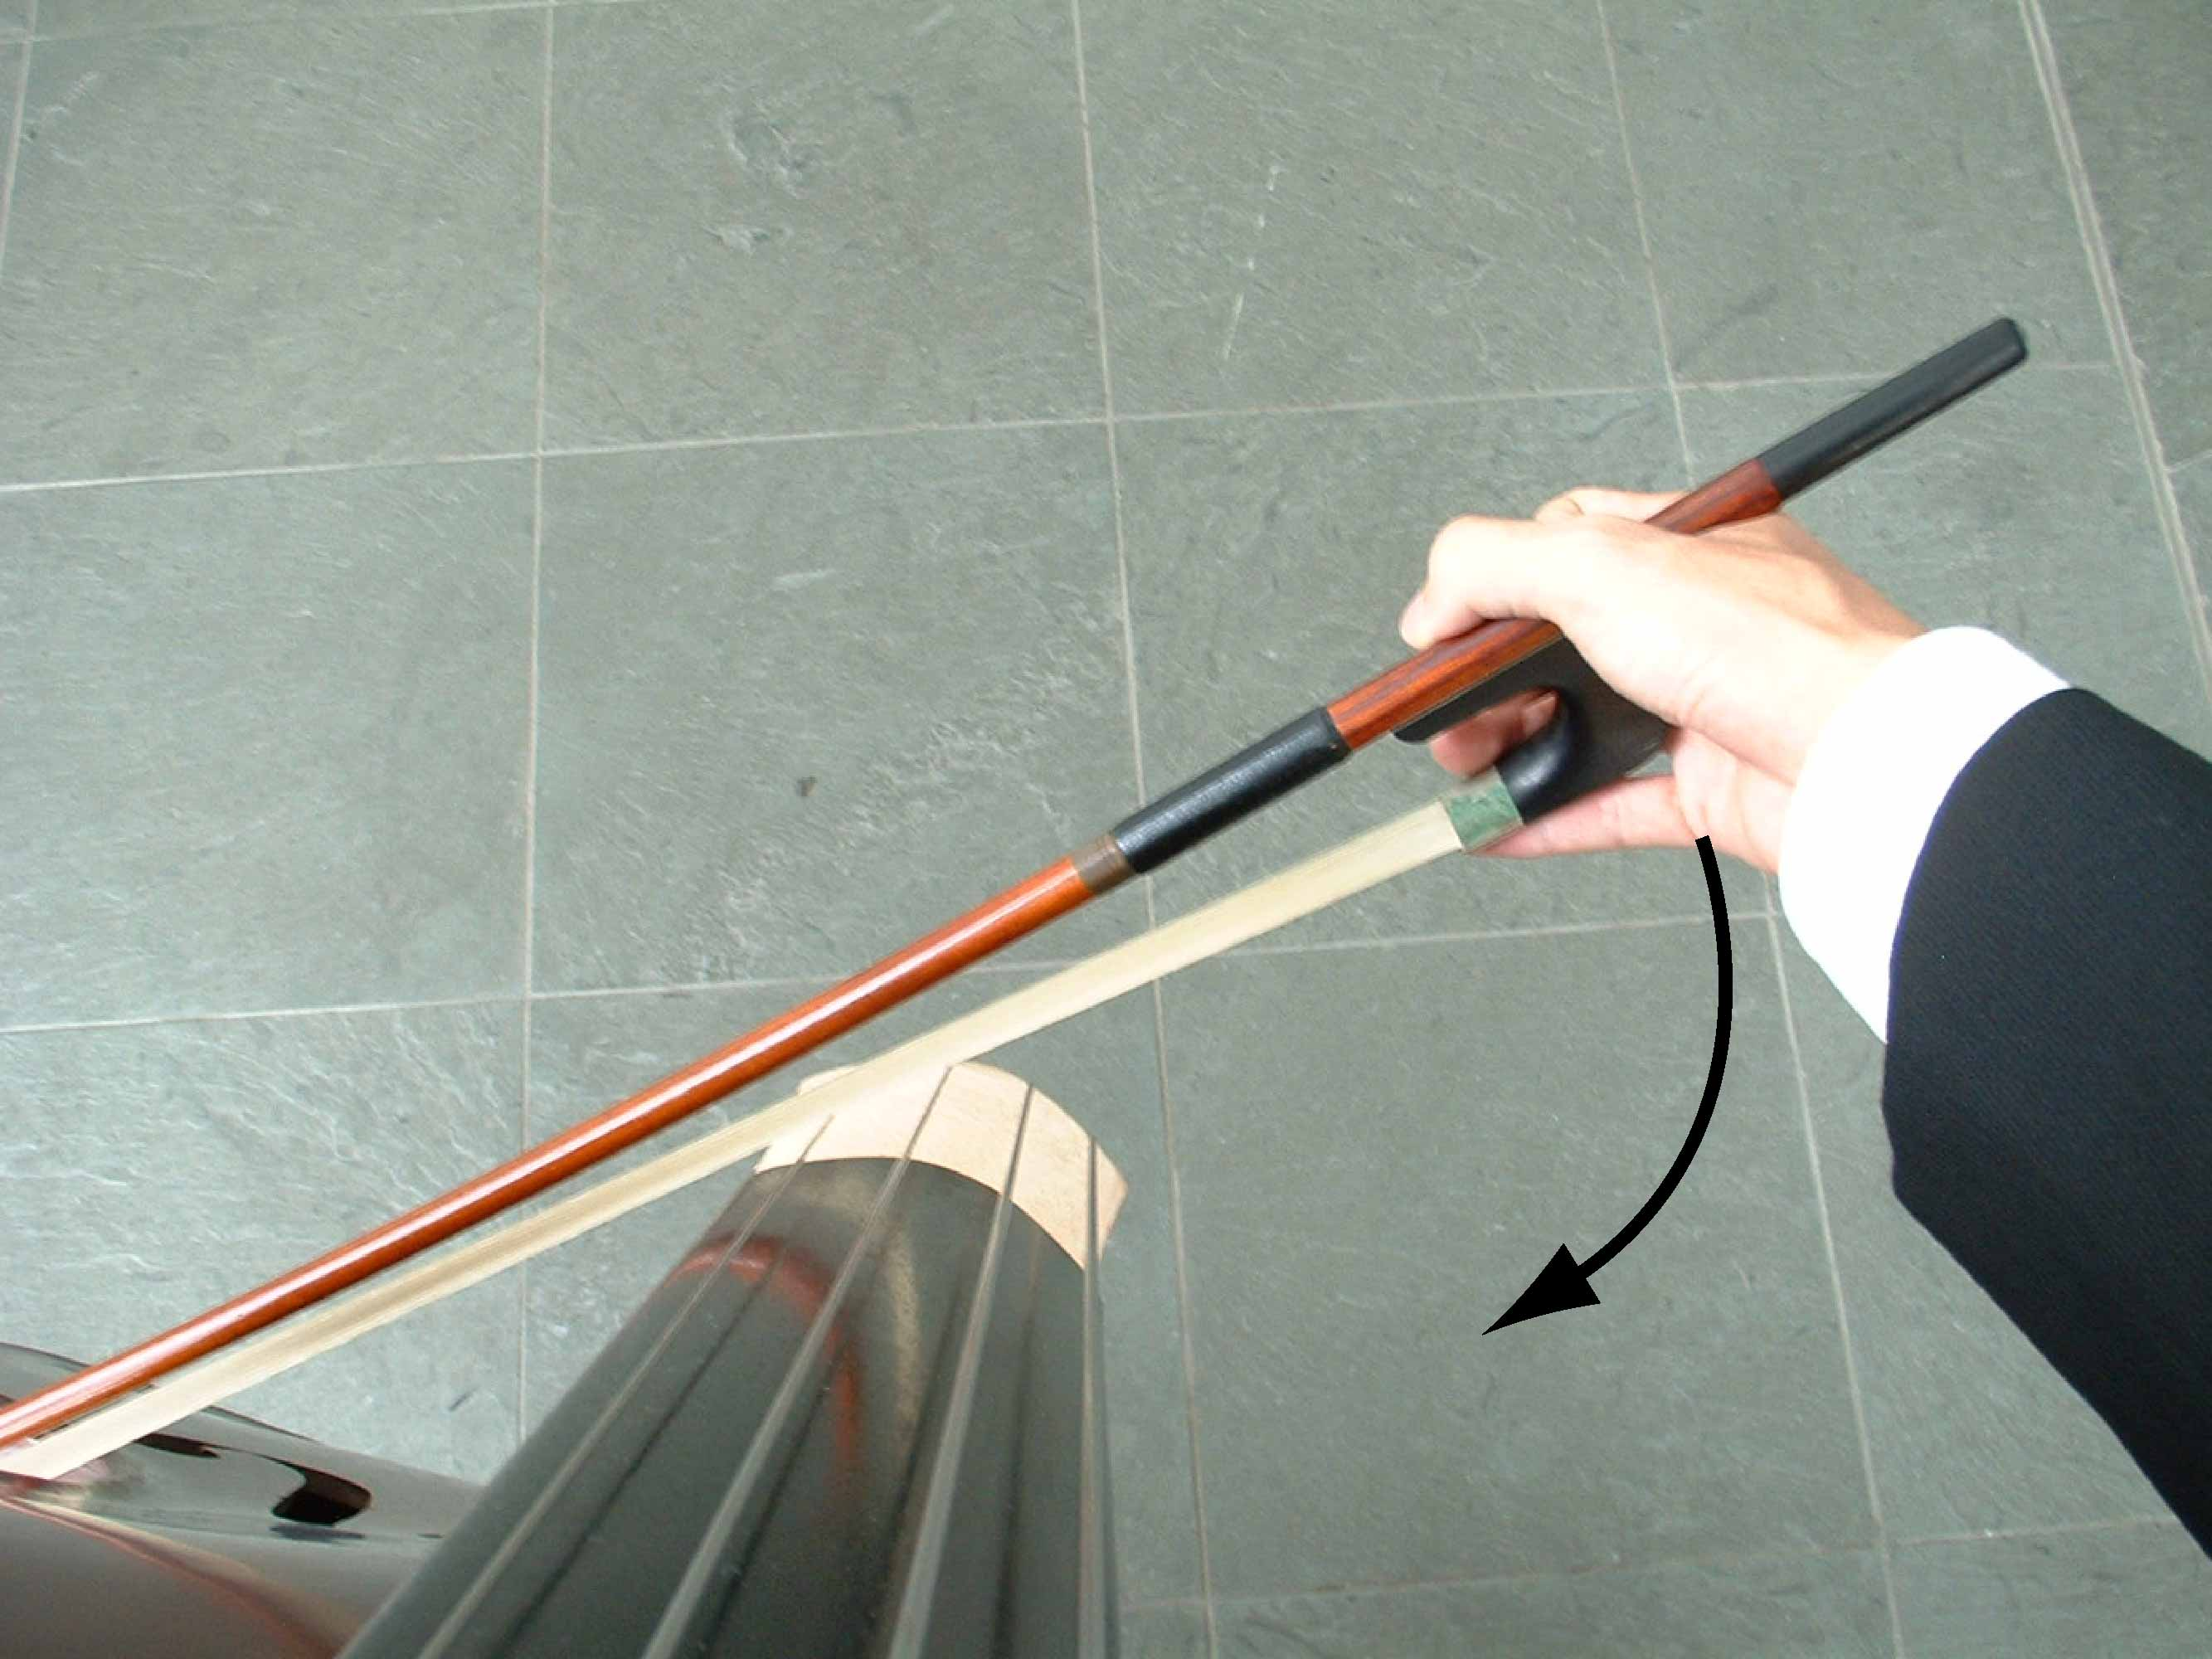
\includegraphics[height=3.8cm]{Pics/photo0830/strchg1.epsi}\\
\addtocounter{figure}{1}
{\small 図\thefigure : 手首を矢印の方向に持って行く\\}
\end{center}
\end{minipage}
\hfill
\begin{minipage}{200pt}
\begin{center}
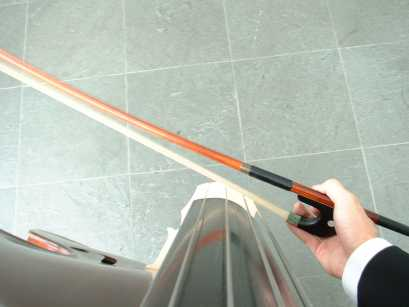
\includegraphics[height=3.8cm]{Pics/photo0830/strchg4.epsi}\\
\addtocounter{figure}{1}
{\small 図\thefigure : 移弦完了\\}
\end{center}
\end{minipage}

\subsection{手首の使い方 \label{wrist}}
音符と音符の間に隙間ができるもう1つの理由に、弓の折り返しがあります。弦上を動きだした弓はやがて末端(弓先か弓元)にたどり着きます。弾き続けるためにはここで折り返して、それまで弓が動いていた方向と逆の方向に弓を動かす必要があります。こうした弓の往復運動を円滑に行う際に重要なのが右手首の動きです。ダウン・ボウからアップ・ボウに移行するには以下のようにします。\\

\begin{quote}
\begin{enumerate}
\item ダウン・ボウで弾き始める
\item 弓先に近付く(図\addtocounter{figure}{1}\thefigure )
\item ダウン・ボウで弾き続けながら手首を内側に向かって突き出す(図\addtocounter{figure}{1}\thefigure )
\item 弓先に到達
\item アップ・ボウ動作の開始
\end{enumerate}
\end{quote}
\ \\
\begin{minipage}{200pt}
\addtocounter{figure}{-1}
\begin{center}
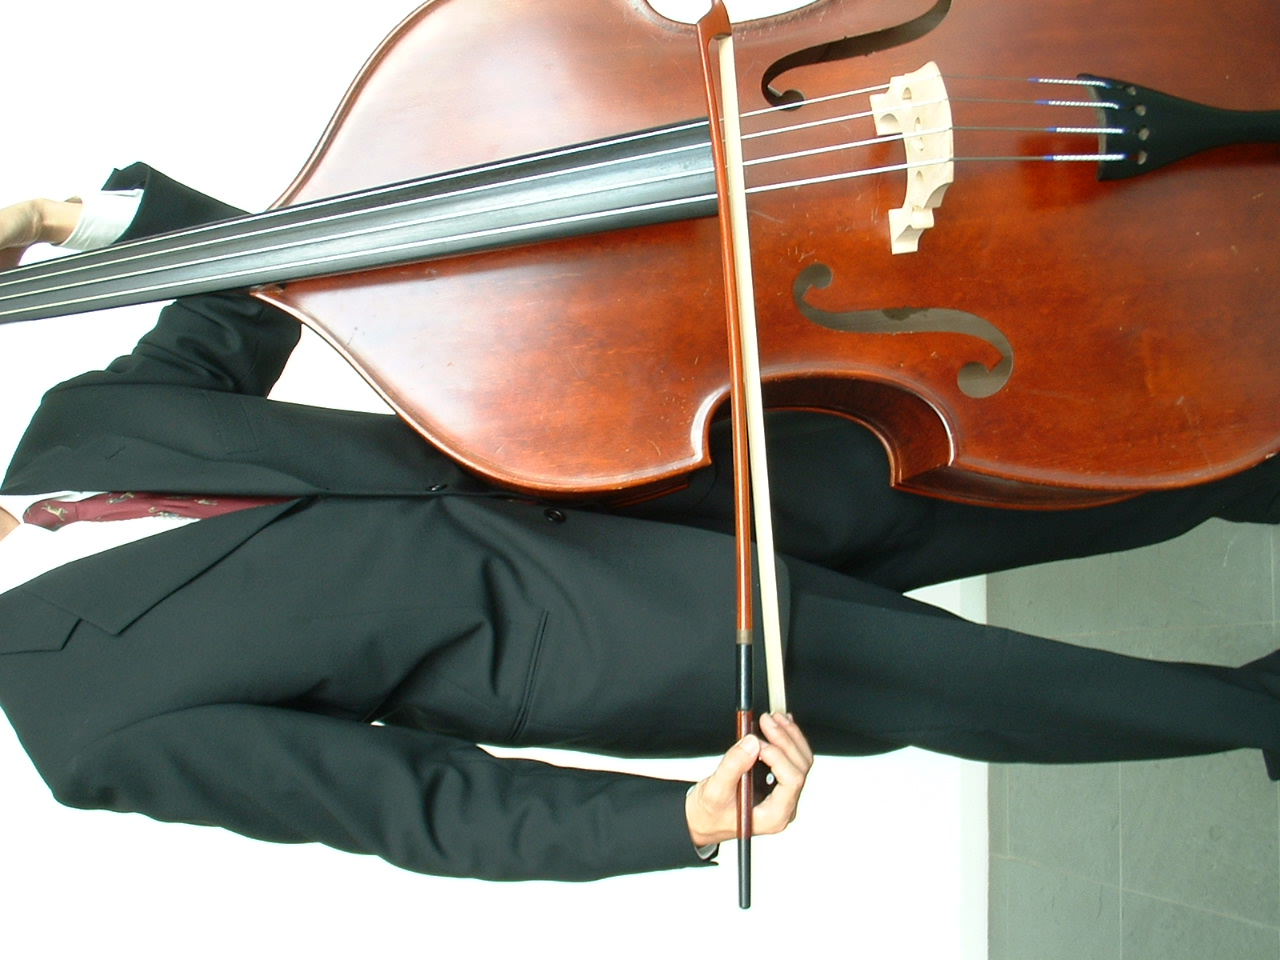
\includegraphics[height=6cm]{Pics/newphoto/bowing1.epsi}\\
{\small 図\thefigure : 弓先が近付く\\}
\end{center}
\end{minipage}
\hfill
\begin{minipage}{200pt}
\addtocounter{figure}{1}
\begin{center}
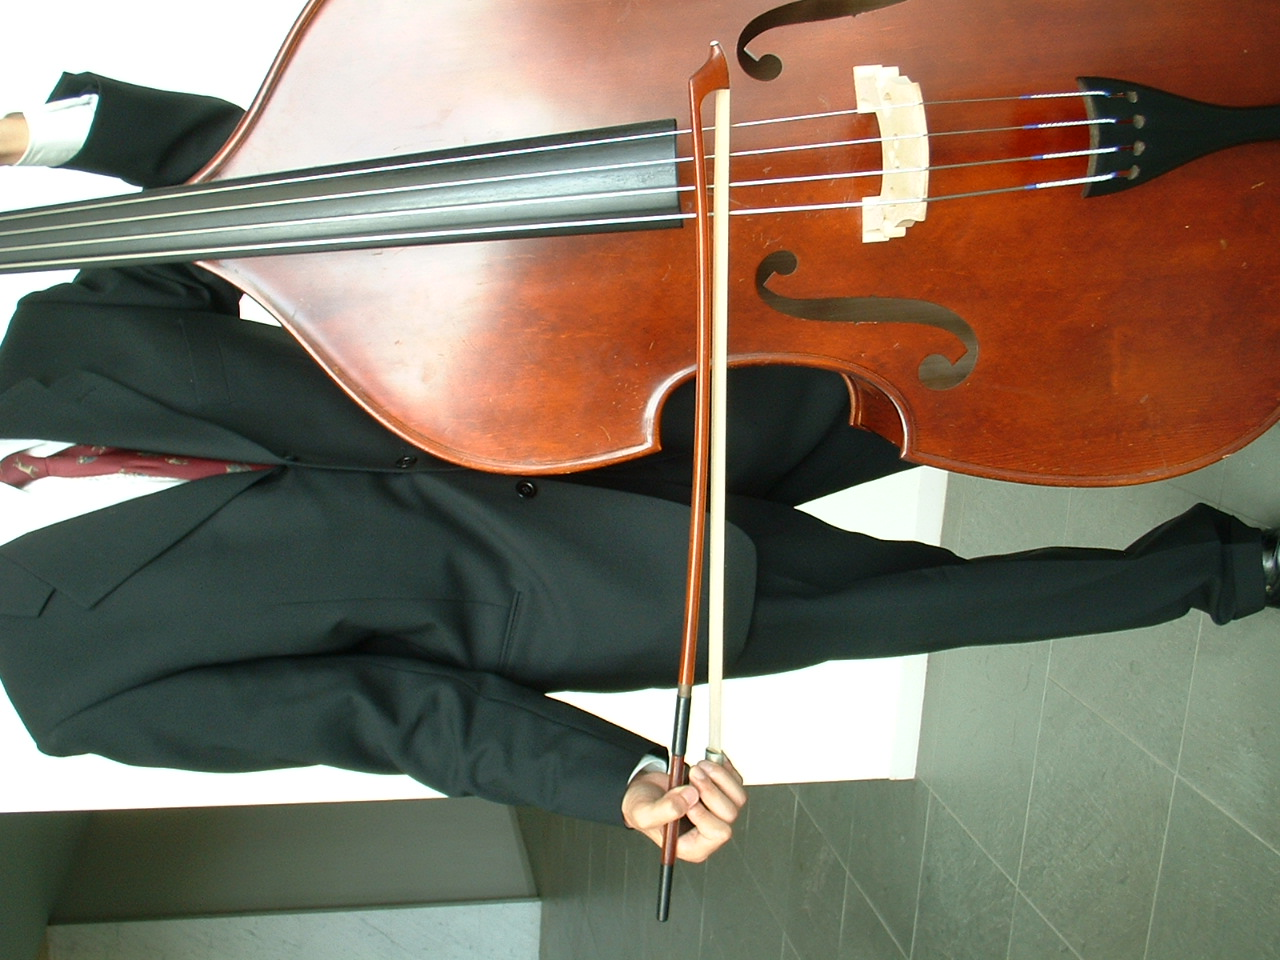
\includegraphics[height=6cm]{Pics/newphoto/bowing2.epsi}\\
{\small 図\thefigure : 手首を内側に入れる\\}
\end{center}
\end{minipage}

\ \\
\indent 逆にアップ・ボウからダウン・ボウに移行するには次のようにします。

\begin{quote}
\begin{enumerate}
\item アップ・ボウで弾き始める
\item 弓元に近付く(図\addtocounter{figure}{1}\thefigure )
\item アップ・ボウで弾き続けながら、内側に突き出していた手首をゆっくり戻す(図\addtocounter{figure}{1}\thefigure )
\item 弓元に到達
\item ダウン・ボウ動作の開始
\end{enumerate}
\end{quote}

\begin{minipage}{200pt}
\addtocounter{figure}{-1}
\begin{center}
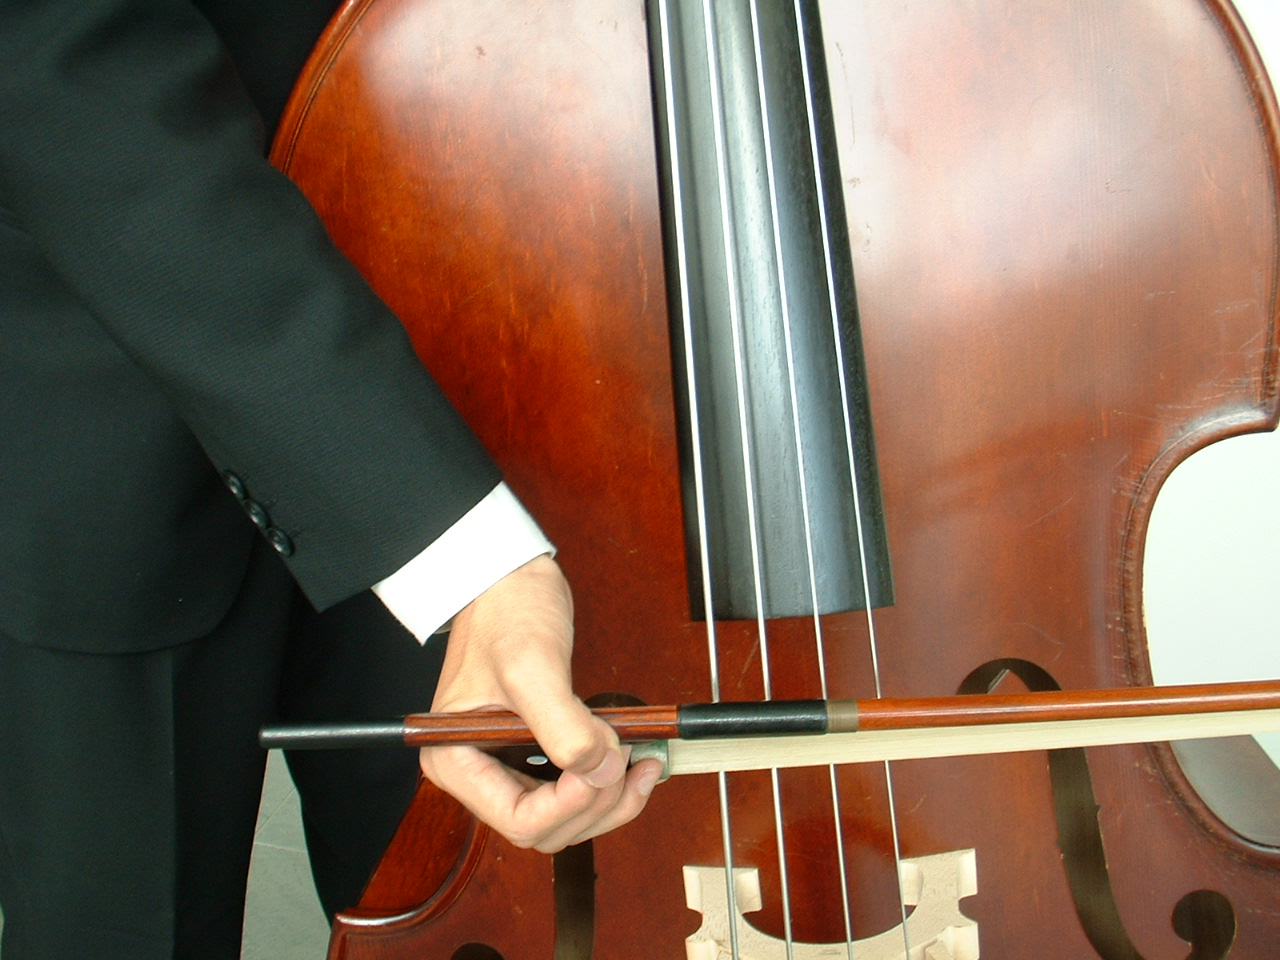
\includegraphics[height=5.4cm]{Pics/newphoto/bowing4.epsi}\\
{\small 図\thefigure : 弓元が近付く\\}
\end{center}
\end{minipage}
\hfill
\begin{minipage}{200pt}
\addtocounter{figure}{1}
\begin{center}
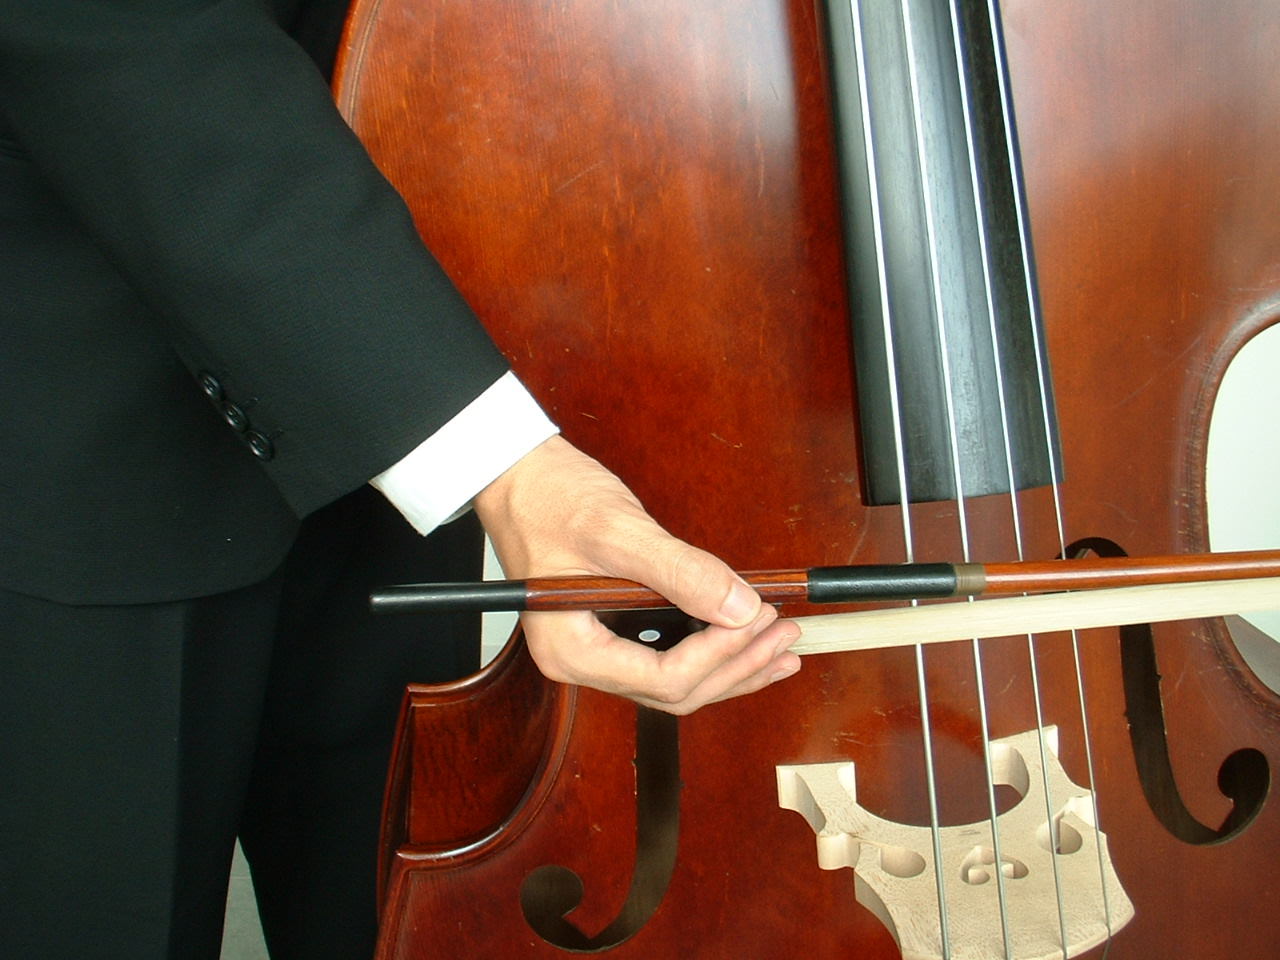
\includegraphics[height=5.4cm]{Pics/newphoto/bowing3.epsi}\\
{\small 図\thefigure : 内側に突き出していた手首を戻す\\}
\end{center}
\end{minipage}

\ \\

最初のうちは弓を折り返した際に弦の振動が止まるか減衰してしまうと思いま
すが、習得に比較的時間がかかる技術ですので焦る必要はありません。毎日の
基礎練習の中で少しずつ取り組んで下さい。弓を折り返しても弦の振動が持続
できるまでになれば、弓の円滑な往復運動をマスターしたと言えるでしょう。

\clearpage

\subsection{開放弦の練習 \label{open2}}
「\ref{strchg}」「\ref{wrist}」で紹介した移弦の方法、手首の使い方を踏
まえて、音符と音符との間に音が鳴っていない時間ができないように開放弦の
練習をしてみましょう。今後、開放弦の練習をするときには、必ず以下の3項
目を点検しながら練習するようにします。

\begin{enumerate}
\item 音量は均一か
\item 手首が柔らかく動いているか
\item 音符の間に音が鳴っていない時間はないか
\end{enumerate}

\begin{music}
\nostartrule
\parindent 0pt
\setclef1{\bass}  
\generalmeter{\meterC}
\startpiece
\notes\zchar{14}{(\metron{\qu}{60})}\enotes
\NOtes\zchar{9}{\downbow}\wh{'D}\enotes
\bar
\notes\enotes
\NOtes\zchar{9}{\upbow}\wh{'A}\enotes
\bar
\notes\enotes
\NOtes\wh{'D}\enotes
\bar
\notes\enotes
\NOtes\wh{'G}\enotes
\bar
\notes\enotes
\NOtes\wh{'A}\enotes
\bar
\notes\enotes
\NOtes\wh{'D}\enotes
\bar
\notes\enotes
\NOtes\wh{E}\enotes
\bar
\notes\enotes
\NOtes\wh{'A}\enotes
\endpiece

\startpiece
\notes\enotes
\Notes\zchar{9}{\downbow}\hl{'D}\zchar{9}{\upbow}\hl{D}\enotes
\bar
\Notes\hu{'A}\hu{A}\enotes
\bar
\Notes\hl{'D}\hl{D}\enotes
\bar
\Notes\hl{'G}\hl{G}\enotes
\bar
\Notes\hu{'A}\hu{A}\enotes
\bar
\Notes\hl{'D}\hl{D}\enotes
\bar
\Notes\hu{E}\hu{E}\enotes
\bar
\Notes\hu{'A}\hu{A}\enotes
\endpiece

\startpiece
\notes\zchar{9}{\downbow}\ql{'D}\zchar{9}{\upbow}\ql{DDD}\enotes
\bar
\notes\qu{'AAAA}\enotes
\bar
\notes\ql{'DDDD}\enotes
\bar
\notes\ql{'GGGG}\enotes
\bar
\notes\qu{'AAAA}\enotes
\bar
\notes\ql{'DDDD}\enotes
\bar
\notes\qu{EEEE}\enotes
\bar
\notes\qu{'AAAA}\enotes
\rightrepeat
\Notes\wh{'D}\enotes
\setdoublebar
\endpiece
\end{music}

\begin{flushleft}
\begin{minipage}{200pt}
\subsection{ピッツィカート(伊 pizzicato)}
\ \ \ \ 譜面上にpizz.と書いてあったら、それ以降の音符は右手の指で弦を
はじいて演奏します。これをピッツィカート奏法と呼びます。ピッツィカート
はarcoと書かれている地点まで続きます。arco以降は元通り弓で演奏します。
強いピッツィカート音を出したいときは人さし指と中指の2本で、小さい音が
欲しいときは人さし指1本ではじきます。
\end{minipage}
\hfill
\begin{minipage}{60pt}
\begin{center}
\addtocounter{figure}{1}
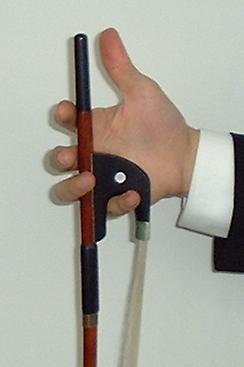
\includegraphics[height=4.5cm]{Pics/Pizz/pizz_1.epsi}\\
図\thefigure \\
\end{center}
\end{minipage}
\hfill
\begin{minipage}{90pt}
\begin{center}
\addtocounter{figure}{1}
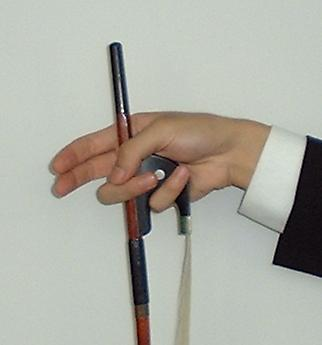
\includegraphics[height=4.5cm]{Pics/Pizz/pizz_2.epsi}\\
図\thefigure \\
\end{center}
\end{minipage}
\end{flushleft}

\begin{minipage}{100pt}
\begin{center}
\addtocounter{figure}{1}
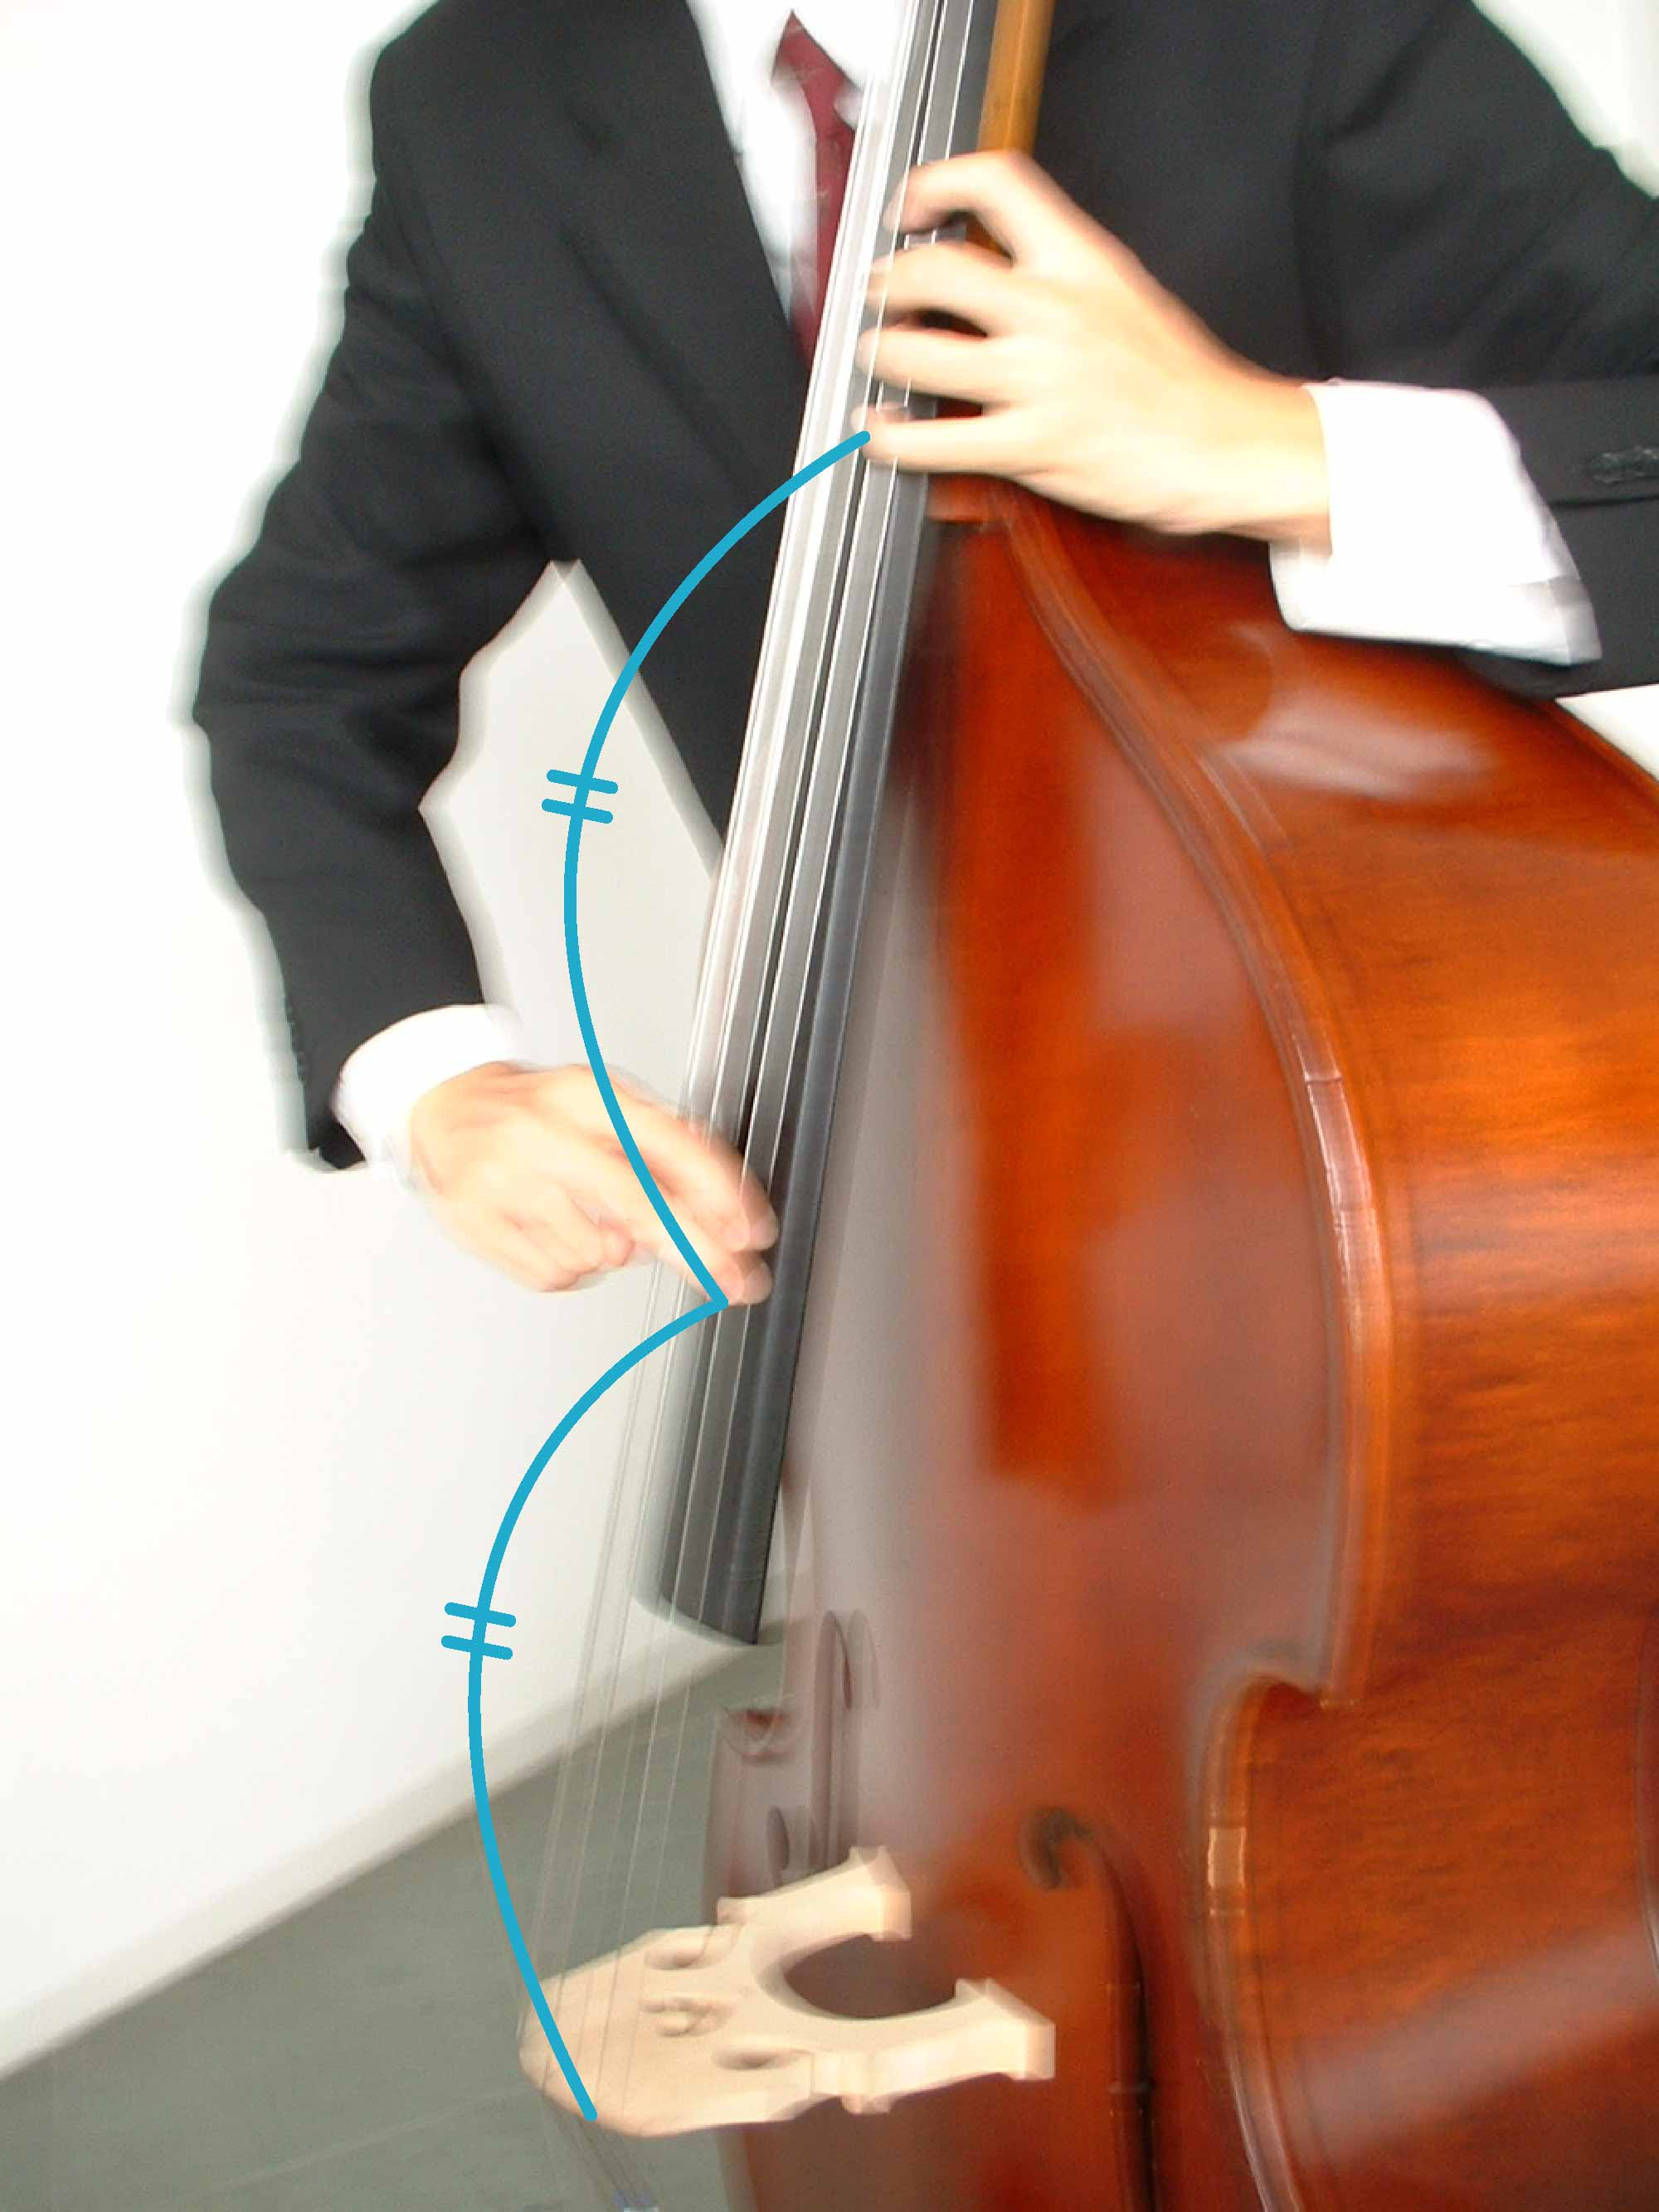
\includegraphics[height=4.5cm]{Pics/photo0830/pizz_point.epsi}\\
図\thefigure \\
\end{center}
\end{minipage}
\hfill
\begin{minipage}{100pt}
\begin{center}
\addtocounter{figure}{1}
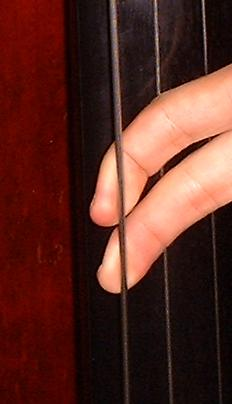
\includegraphics[height=4.5cm]{Pics/Pizz/pizz_3.epsi}\\
図\thefigure \\
\end{center}
\end{minipage}
\hfill
\begin{minipage}{220pt}
\begin{center}
\addtocounter{figure}{1}
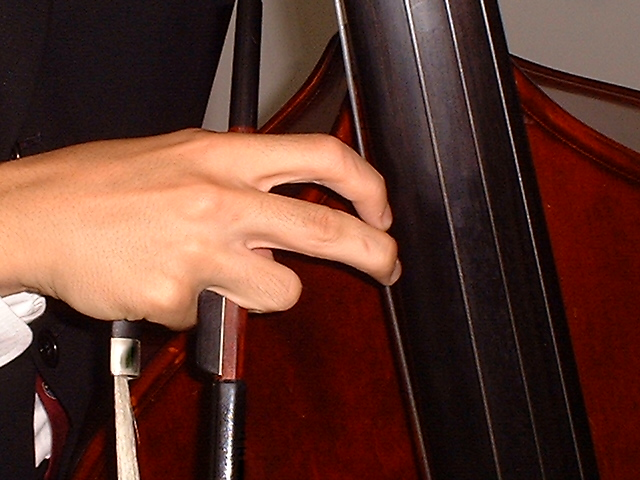
\includegraphics[height=4.5cm]{Pics/Pizz/pizz_4.epsi}\\
図\thefigure \\
\end{center}
\end{minipage}

\begin{enumerate}
\item まず小指に弓を引っ掛けます(\addtocounter{figure}{-4}図\thefigure )。
\item 弓を握ります(\addtocounter{figure}{1}図\thefigure )。
\item 左手で押さえた地点から駒までの中間点に右手の指を持って行きます(\addtocounter{figure}{1}図\thefigure )。
\item 指を弦に押し当て、指先に「肉溜まり」をつくります(\addtocounter{figure}{1}図\thefigure )。
\item 弦を横方向に引っ張ります(\addtocounter{figure}{1}図\thefigure )。
\item 弦を放し、エネルギーを一気に開放します。弦を指板に当てて雑音を出さないように注意しましょう。
\end{enumerate}

\subsection{ベース椅子とその座り方}

\begin{minipage}{200pt}
\ \ \ \ \ コントラバスは立っても座っても演奏できます。座って演奏する場合には
\addtocounter{figure}{1}図\thefigure のような「ベース椅子」または「バス椅子」と呼ばれる高椅子に座ります。ベース椅子に座る際には\addtocounter{figure}{1}図
\thefigure のように左足を踏み台にかけ、右足を伸ばします。

\addtocounter{figure}{-1}
\begin{center}
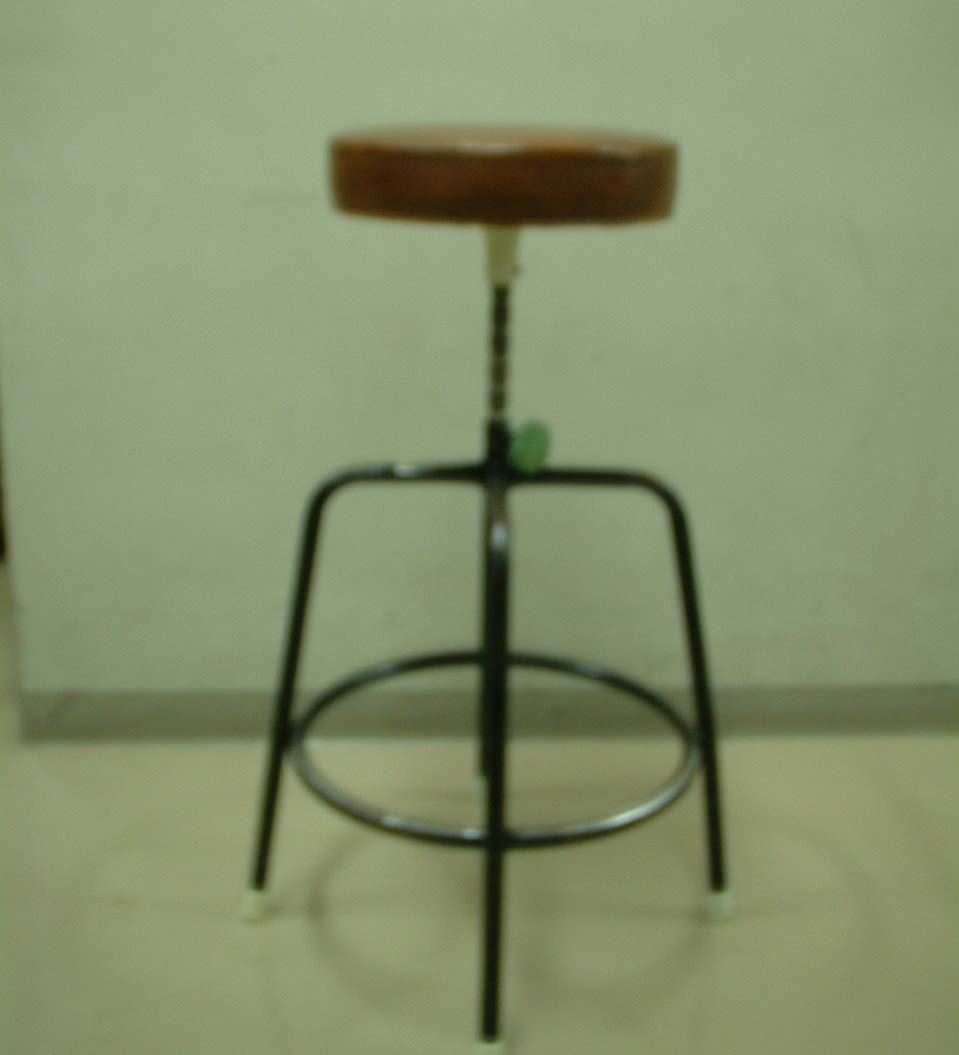
\includegraphics[width=2.3cm]{Pics/newphoto/chair1.epsi}\\
{\small 図\thefigure : 典型的なベース椅子\\}
\end{center}
\end{minipage}
\hfill
\begin{minipage}{120pt}
\addtocounter{figure}{1}
\begin{center}
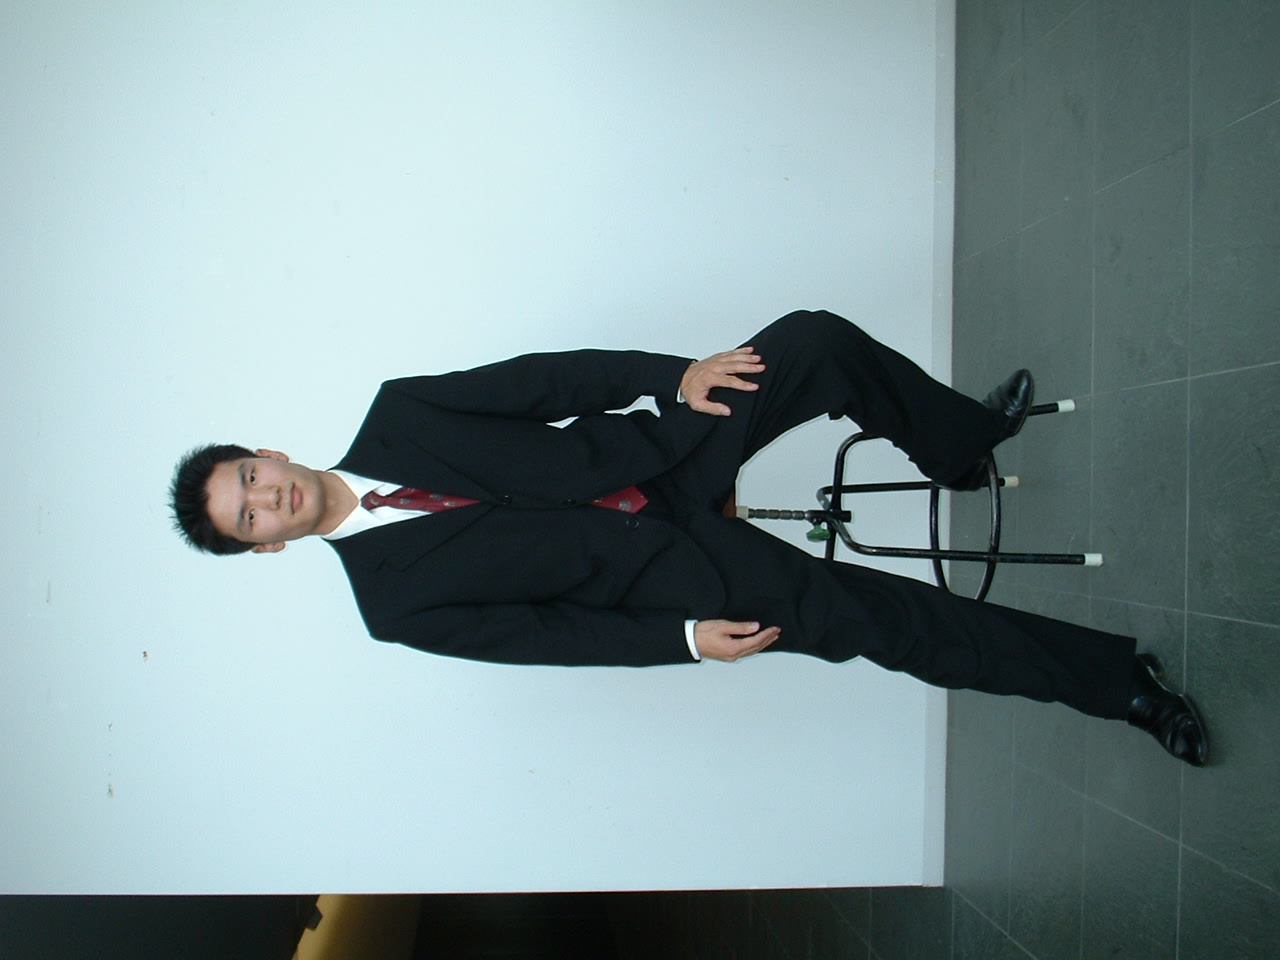
\includegraphics[height=6.5cm]{Pics/newphoto/chair2.epsi}\\
{\small 図\thefigure : 左足を踏み台にかける\\}
\end{center}
\end{minipage}
\hfill
\begin{minipage}{100pt}
\begin{center}
\includegraphics[height=6.5cm]{Pics/newphoto/chair3.epsi}\\
\addtocounter{figure}{1}
{\small 図\thefigure : 楽器を体に預ける\\}
\end{center}
\end{minipage}

\begin{minipage}{190pt}
\begin{center}
\includegraphics[height=5.8cm]{Pics/photo0830/sit_left.epsi}\\
\addtocounter{figure}{1}
{\small 図\thefigure : 左側から\\}
\end{center}
\end{minipage}
\hfill
\begin{minipage}{130pt}
\begin{center}
\includegraphics[height=5.8cm]{Pics/photo0830/sit_back.epsi}\\
\addtocounter{figure}{1}
{\small 図\thefigure : 背面から\\}
\end{center}
\end{minipage}
\hfill
\begin{minipage}{100pt}
\begin{center}
\includegraphics[height=5.8cm]{Pics/photo0830/sit_right.epsi}\\
\addtocounter{figure}{1}
{\small 図\thefigure : 右側から\\}
\end{center}
\end{minipage}


\clearpage
